\documentclass[../MAIN.tex]{subfiles}
\begin{document}
\ro{Rozdział I\\
Wieść:}  
% 
Wskazówki kieszonkowego chronometru ustawiły się prostopadle demonstrując tym samym kwadrans po dwunastej. Trwającą dotychczas ciszę zakłócił zgiełk i hałas zasuwanych krzeseł. Spiker przez megafon donośnie ogłosił przerwę w pracy. Giennadij schował podarowany niegdyś przez ojca zegarek do jednej z kieszeni uniformu i wstając zakomunikował woźnemu koniec pełnionej funkcji. Zanim ruszył do wyjścia złączył plik kartek i starannie umieścił go w szufladzie, po czym delikatnym ruchem ręki umieścił kluczyk w zamku, mechanizm matowo szczęknął tym samym zabezpieczając wartościowe dokumenty przed wścibskim okiem osób trzecich. Giennadij zasunął fotel i skierował się do wyjścia. 
\sx
Jak panu czas mija? -- odezwał się woźny kręcąc kluczami. 
\xx Wyjątkowo szybko, dzisiaj akurat mało roboty i można trochę poleniuchować za biurkiem -- odpowiedział Giennadij wyciągając z torby śniadanie. 
\xx Widzi Pan, ja nawet nie mogę nóg wyłożyć na taboret, bo zaraz przyleci kierownik i opieprzy. Ostatnio to mi krzyżówki zabrał dziadyga jeden, was to tam nie pilnują, bo robota inna, ale mnie od razu za uszy ciągną. 
\xx A ja panu powiem, że papierkowa robota też za ciekawa nie jest w dodatku muszę zajmować się obserwacją i pomiarem próbek. Czasami zamienił bym się z kimś pracą, tak dla odmiany -- uśmiechnął się Giennadij i pozdrawiając kolegę udał się do jadalni. 
\qd
W ciągu paru minut salę wypełnił cały personel, panujący gwar nosił się po ścianach tworząc przenikliwe echo. Giennadij idąc korytarzem co rusz witał pozostałą personę, która z przejęciem pałaszowała wymyślne dania sporządzone przez siebie lub rodzinę. Pracownik postanowił przysiąść się do kolegów z kadry. 
\sx
Cześć Gieno, co tam Ci dziś żonka sprezentowała, moja się pofatygowała i jabłecznik upiekła -- rzucił starszy przyjaciel, na, którego wszyscy wołali Wuser. 
\xx Kanapki z szynką i ogórkiem, nic szczególnego -- pochwalił się Giennadij rozwijając papier z pieczywa. 
\xx No widzisz, trzeba się postarać w nocy, by rano dostać taki specjał -- zaśmiał się Wuser odsłaniając zęby pełne ciasta. 
\qd
Wszyscy obok zrobili to samo, o mało się nie krztusząc. Brechtające gęby nagle umilkły, gdy obiekt żartów wyciągnął zza pazuchy buteleczkę. Wszyscy zrobili konspiracyjne miny i po chwili ponownie zarechotali strojąc przy tym komiczne miny. Wszyscy z aprobatą przyjęli pomysł strzelenia przysłowiowego kielicha i potajemnie wyciągnęli w stronę Giennadija kubeczki z termosów. Kieliszków nikt nie nosił z obawy przed kontrolą, samo noszenie napojów alkoholowych do pracy mogło przynieść za sobą poważne konsekwencję. Jednak koneksje z pracownikami wyższego szczebla dawały gwarancję na przymrużanie oka w przypadku sytuacji łamiących regulamin, a takowe układy posiadał Giennadij. 
\sx
Może kawałek ciasta? Śmiało częstować się -- oznajmił Wuser, wpychając do ust kolejną porcję jabłecznika. 
Zgromadzeni przy stole przyjęli podarek w ciszy delektując się słodkim deserem. 
\xx Słyszeliście o pewnej rekrutacji, którą mają tutaj wdrożyć. Ponoć tajne ugrupowanie zbiera ludzi do bliżej nieokreślonych prac związanych z badaniem promieniowania w Czarnobylu. Wiadomo mi, że inicjatorem tego przedsięwzięcia ma być niejaki Piotr Kaługin. Słyszeliście o takim? -- zapytał Wuser robiąc przy tym kwaśną minę. 
\xx Nie znam gościa, pewnie jakiś świr. Ciekaw jestem co oni chcą badać w tym wyludnionym mieście zawalonym kupą stali i innymi rupieciami -- wtrącił inny kolega z personelu. 
\xx Mi to wygląda na jakiś zakulisowy program. Przecież u nas w Prypeci prowadzimy diagnozy nad oddziaływaniem promieniowania na tutejszą florę i faunę, więc dlaczego mieliby to samo robić w Czarnobylu. Może środowisko inne i badania ciekawsze. Jeśli mnie wybiorą to z chęcią zmienię otoczenie, może lepiej płacić będą -- dodał i uśmiechnął się półgębkiem Patejuk 
\xx A ty Giennadij co o tym sądzisz? -- rzucił ponownie Wuser ignorując ostatnią wypowiedź. 
\xx Ciekaw jestem co z tego wyniknie. Zastanawiam się, gdzie oni prowadzaliby te doświadczenia, bo chyba nie na wolnym powietrzu. Może w planach mają budowę kompleksu badawczego, tylko że postawienie takiego ośrodka to nie bagatela. Prace budowlane zajęłyby co najmniej dwa lata. 
\xx Według mnie wszystko jest już przygotowane, skoro ewentualna rekrutacja ma się niebawem odbyć. W ogóle skąd wiesz o tej całej akcji? -- spytał Patejuk.
\qd
Wuser otworzył lekko usta, lecz nic z nich nie wydobył. Wziął do ręki kubek z kawą i zakręcił, nim mieszając resztki czarnego naparu. Zwięzłe milczenie przerwała fonia dzwoniącej aparatury głosząc tym samym koniec przerwy. 
% 
\sx Kierownik wspominał, ale jak, by co gębą na kłódkę. Nie warto rozpowiadać, bo się rozejdzie po całym zakładzie i się zamęt zrobi. To do jutra! -- zakomunikował Wuser i odszedł od stołu zabierając torbę. 
\qd
Patejuk z resztą kadrowiczów postąpił tak samo.

Przy stole został tylko Giennadij, w tle cichły ostatnie rozmowy i odgłosy kroków. Salę ogarnęła osobliwa atmosfera. Strzeliste białe ściany piętrzyły się przed wzrokiem osamotnionego pracownika, a silny blask jarzeniówek potęgował dziwną aurę. Pomieszczenie wyglądało teraz jak wielka poczekalnia, a osoba siedząca w centrum była jak ostatnia dusza na ziemi będąca na łasce kapryśnego stwórcy wahającego się przed wyborem -- ukarać czy ocalić przed wiecznym potępieniem. Zamyślony Giennadij wyrwał się z letargu poruszony jakąś niewidzialną siłą. Zdając sobie sprawę, że przerwa dawno minęła pośpiesznie zerwał się na nogi i w żwawo ruszył do wyjścia. W jego umyśle zagnieździła się nowina na temat rekrutacji i stała się bodźcem do dalszych przemyśleń o ewentualnej zmianie pracy. Zegar wskazywał godzinę dwunastą trzydzieści.
%
\clearpage
\ro{Rozdział II\\ Gość:}  
% 
Za oknem panowała okropna szaruga, intensywny wiatr szarpał nagie gałęzie i w wirującym rytmie miotał zżółkłymi liśćmi. Niebo okryło się ciemną kłębiastą szatą nie pozwalając rzucić jakiegokolwiek promyku na jesienną ziemię. Marna pogoda i ponura sceneria z betonu odbierała wszystkim witalności i wprawiała w przygnębienie. Gęsty nastrój za ścianami ośrodka badawczego nie przeszkadzał jednak nikomu w codziennej pracy. Giennadij w swoim gabinecie analizował rośliny poddane radiacji, próbki różnej wielkości miały swoją unikalną sygnaturę i oddzielną charakterystykę w notatkach. Egzemplarze dostarczano z Czerwonego Lasu, gdzie flora przeszła największą mutację. 

Doświadczony naukowiec wyciągnął zza ucha długopis i zaczął kreślić wymyślne symbole w ramkach podręcznego notesu, żmudną pracę zakłóciło pukanie do drzwi. 
-- Witaj, zajmę Ci tylko chwilę. Mam nadzieje, że nie przeszkadzam. Dzisiaj około piętnastej przyjdą ci od rekrutacji. Powiedziałem kierownictwu, żeby nowo przybyli goście rozpatrzyli twoją kandydaturę. Oczywiście żadnych oficjalnych wniosków o posady nie było, ale jak, by, co to się piszesz, no to trzymaj się -- Wuser kiwnął głową i zamknął drzwi za sobą. 
Giennadij nie zdążył nawet podziękować. Ucieszył się z faktu, że może zostać przeniesiony i poszerzyć swoje horyzonty, ale jednocześnie dziwił się czemu Wuser tak bardzo troszczy się o jego zawód. Nie marnując czasu wrócił do poprzedniego zajęcia. W jednym z protokołów napisał:\\
% 
\texttt{Próbka numer [3] \textit{Populus Nigra} wyraźnie wykazuje wzmożone zdolności regeneracyjne. Ociosany pień po, zaledwie dwóch dniach wraca do pierwotnej postaci; słabo widoczne ślady okaleczenia rośliny. Komórki kambium zmieniły swoją wewnętrzną strukturę w wyniku przyjęcia wysokiej dawki promieniowania. Przyspieszona ekwipotencjalność oznacza brak zagrożenia przed czynnikami patogennymi. Liście \textit{Populus Nigra} zawierają stosunkowo duże ilości niezidentyfikowanej do końca substancji, przypuszczalnie mogą to być neurotoksyny; planowane doświadczenie na szczurach. Zaobserwowano niską wodochłonność. Dalsze eksperymenty wykażą czy badana \textit{Populus Nigra} może zostać uznana jako nowy gatunek.} 

Przelany na arkusze papieru wynik doświadczeń został zapisany również w formie nagrania. Giennadij wszelki rezultat swojej pracy przechowywał w postaci cyfrowej, lubił mieć wszystko w jednym miejscu na małym mobilnym dysku. Młody naukowiec usiadł na obitym skórą fotelu robiąc sobie krótką przerwę od zajęć. Ziewnął przeciągle drapiąc się za uchem. Wyciągnął z kieszeni swój poczciwy zegarek i określił czas dzielący go od rzekomej wizyty ludzi od rekrutacji. Pozostały dwa kwadranse, bezczynne oczekiwanie sprawi, że czas na złość mijać będzie wolniej. Inercji w pracy Giennadij unikał jak ognia, więc postanowił zająć się czymkolwiek, padło na czyszczenie sprzętu laboratoryjnego. 

Po, zaledwie kilku minutach wszystkie probówki o różnorakiej wielkości i wymyślnych kształtach błyszczały pod ostrym światłem lamp żarowych. Giennadij mył właśnie ręce, gdy do drzwi zapukała tajemnicza osoba. 
\sx
Witam. Nazywam się Stiepan Sewienkov. Pan nie musi się przedstawiać. Zapewne, domyślacie z jakiej racji się tu zjawiłem. Pozwolicie, że opuścimy gabinet i udamy się do specjalnego pokoju, gdzie omówimy ważne sprawy -- oznajmił i gestem grzecznościowym wskazał drzwi wyjściowe -- Pańskie dokonania zrobiły na nas duże wrażenie i nie ukrywam, że biogram jest gwarantem nowej posady.
\qd
Giennadij nieco speszony milczał, ale uważnie słuchał hipnotyzującego głosu, na potwierdzenie słów kiwał tylko głową. 
\sx Procedury wymuszają na mnie zadanie pytania, które zapewni dalsze postępowanie wobec badacza. Podjęcie nowej pracy będzie się wiązało z poufnością. Badania przeprowadzane w Strefie są ściśle tajne i tylko kilkanaście osób wie o ich działaniu, akredytując przedstawione warunki automatycznie wyraża pan zgodę na trzymanie w tajemnicy wyników pracy. Więc jak? Odmowa sprawi, że zostawię pana tu i teraz, dalsze informacje nie zostaną udzielone. -- rzucił gość robiąc pełne powagi spojrzenie.
\qd
Odbiorca zamyślił się na chwilę. Atmosfera zgęstniała. Tajemnicza postać nieco teatralnie zdjęła okulary i odsapnęła aluzyjnie wymuszając na badaczu podjęcie ostatecznej decyzji. Giennadij czuł na ciele dreszcz i nietypowe podniecenie przed czymś nowym, nieznanym. Sytuacja nie była do końca jasna, akceptacja warunków postawionych przez Sewienkowa wiązała się z pewnymi ograniczeniami. Odmowa nie wchodziła w grę, Giennadij był za bardzo podekscytowany i ciekawy projektu, którego miał być świadkiem, a jednocześnie ciężko mu było wyjść z klinczu i po prostu odpowiedzieć z aprobatą i rozwiać wszelkie wątpliwości. Wyraźnie czuł jak chłodne krople potu przemieszczają się po jego ciele, wzrok cierpliwego przybysza zdawał się oddziaływać coraz mocniej. Każda ulatniająca się sekunda sprawiała, że w oczach przyszłego pracodawcy naukowiec wyrastał na błazna i niezdecydowanego dzieciaka, który nie wie o jakim smaku lizaka chce dostać. Giennadij musiał podjąć finalną decyzję. 
% 
\sx Przyjmuję propozycję -- wyrzucił w końcu młody badacz. 
\xx Doskonale, lepiej zastanowić się kilka razy niż pochopnie coś postanowić. -- odrzekł powściągliwie i ruszył dalej korytarzem.
\qd
Słowa o lekko sarkastycznym akcencie nie uderzyły w Giennadija. Wnikliwość narastała z każdym pojedynczym cyknięciem sekundnika kieszonkowego zegarku. 
% 
\sx Zapali pan? -- wyrwał nagle gość. 
\xx Nie palę -- odparł standardowo Giennadij. 
\qd
Stiepan za pomocą połyskującej zapalniczki benzynowej zajął papierosa i zaciągnął się ochoczo. Od razu dało się poznać, że Sewienkov jest silnie uzależniony, przysłowiowy dymek sprawiał mu wiele radości i nie dało się tego ukryć. 
% 
\sx Proszę tutaj. Niech pan usiądzie.
\qd
Drzwi za nimi trzasnęły i wszelki hałas dobiegający z korytarza umilkł. Silnie oświetlony gabinet został już wcześniej przyrządzony. Na środku salki znajdował się stolik rozdzielający dwa eleganckie fotele. Dwaj panowie zasiedli przy drewnianej ławie i przystąpili do kontynuowania kontraktu. 
% 
\sx Otrzyma pan teraz kilka formularzy, które wystarczy skwitować podpisem. Streszczę większość stronic, by zaoszczędzić nam czasu. Przypominam, że podjął pan ostateczną decyzję, bez odwołania. Wszelkie próby złamania zaakceptowanych przez pana zasad poniosą za sobą poważne konsekwen\3k Zresztą dorzeczy, darujmy sobie te formułki. Poza panem zostały wybrane także dwie inne osoby, nazwisk zdradzać nie będę, wszystko w swoim czasie. Machnie pan autograf w kilku miejscach i tym samym stanie się pan jednym z elementów naszej układanki. Projekt nosi nazwę "S--01" i jego celem jest stworzenie "unikalnego środka" chroniącego przed bardzo wysokimi dawkami promieniowania. Eksperymenty są niebezpieczne i dlatego potrzebujemy wykwalifikowanych pracowników z doświadczeniem. Tam nie będzie pan obserwował roślinek. Projekt "S--01" to zupełnie inny kaliber. Więcej dowie się pan w najbliższym czasie. 
\xx Od, kiedy zaczynam i co z moją aktualną posadą? -- spytał Giennadij podpisując ostatni dokument 
\xx Jutro o tej samej godzinie zostanie pan przetransportowany na nowe miejsce pracy. Spotkamy się i omówimy jeszcze kilka drobnych spraw. Owoce pańskiej pracy zostaną na miejscu. Jeszcze jakieś pytania? -- Stiepan wstał dogasił papierosa i oczekując odpowiedzi zaczął pakować pliki do aktówki. 
\xx To chyba wszystko. I dziękuje -- Giennadij także wstał wystawiając dłoń w geście pożegnania. 
\xx To ja dziękuje -- gość uścisnął rękę i otwierając na oścież drzwi wpuścił do gabinetu nieco korytarzowej wrzawy.
\qd
Młody naukowiec został sam, ponownie, z kolejną serią dręczących go pytań.
% 
\ro{Rozdział III\\Wola:}  
% 
Telewizor w skromnie urządzonym pokoiku nadawał poranne wiadomości odganiając jednocześnie senną aurę. Na palniku kuchennym swój mały koncert zainaugurował czajnik wydobywając z dziobka sowite ilości pary. Wyrzucony pod wpływem ciśnienia gwizdek poturlał się w stronę drzwi wyjściowych, Giennadij uciszył buchające naczynie i podniósł z podłogi metalowy element. Wrzący strumień wody wypełnił przeźroczysty kubek tworząc brunatny napar. Młody naukowiec zabrał stygnącą herbatą do pokoju, gdzie mógł posłuchać ostatnich wiadomości. Giennadij usadowił się wygodnie w fotelu i wytężył słuch wklejając spojrzenie w ekran. W telewizji przedstawiano właśnie prognozę pogody: 

"\3kw Obwodzie żytomierskim bez opadów, liczne przejaśnienia. Temperatura w granicach pięciu stopni. Natomiast na terenie całego obwodu kijowskiego silny wiatr i ulewa. W północnej części nawet dwa stopnie poniżej zera. Obwód czernihowski za sprawą niżu z nad\3k" 

Odbiornik błyskawicznie zmienił swoje oblicze śnieżąc i wypluwając z głośników jazgoczące dźwięki. Kapryśne ustrojstwo nie milkło i wtórowało przekleństwom rzucanym przez Giennadija. Zapowiadana pogoda najwyraźniej wyrządziła szkody i zerwała gdzieś kable telekomunikacyjne. Naukowiec poruszył kilka razy anteną, lecz w pokoju wciąż rozlegał się ten sam ton. Zirytowany zdławił w sobie złość i odszedł od telewizora, usiadł w fotelu i ciężko westchnął. Miał jeszcze parę minut, ale nie chciał pozostałego czasu przeznaczyć na zajmowanie się płatającym figle odbiorniku. Giennadij wskoczył w buty założył szykowny prochowiec i w zwyczaju zerknął na zegarek. 

Rwący wiatr stał się reżyserem srogiej jesiennej scenerii, ulotna materia w rytmie rozhulanego wichru przemierzała kilometry, nieokiełznane siły natury w akompaniamencie upiornego świstu ciskały liśćmi kreując nieustannie obraz rozległej sfery. Półnagie drzewa urokliwie tańczyły trzymając się chwiejnego taktu, a cienkie gałęzie pod potężnymi podmuchami wyginały się na boki. Mroźny dżdżysty deszcz uderzał w ponurą ziemię przeistaczając się w błotniste kałuże, które topiły w swoim nurcie kruche gałęzie. Pierzaste kłęby zalały bezkres nieba jakby urzeczywistniając wizję szalonego malarza przelewającego na płótno swoje najczarniejsze koszmary. Do nieobliczalnej konfrontacji sił przyrody wdał się piorun rysując na sklepieniu świetliste odnogi. Surowe wycie wiatru okazało się malutkie przy potężnym grzmocie, stukanie kropli i szmer roślin na chwilę ucichł. 
% 
\sx Nie zapowiadali dzisiaj burzy i to z rana, przeczekam tę nawałnicę. -- powiedział sam do siebie, wyjął z płaszcza telefon i z powrotem wszedł do klatki schodowej. 
\qd
W słuchawce rozległo się słabo słyszalne pikanie informujące o braku połączenia. Giennadij powtórzył kilka razy tą samą czynność, lecz bezskutecznie. Niesprzyjające warunki najwidoczniej zakłócały wszelką prace urządzeń falowych. Naukowiec nie mógł zwlekać z przyjazdem do pracy, kierownictwo musi zostać poinformowane o ewentualnym spóźnieniu. Restrykcyjne zasady komplikowały okoliczności w jakich znalazł się Giennadij. Pozostało mu tylko wsiąść do samochodu i jechać w kierunku Prypeci. 

Silnik parokrotnie zaterkotał, po czym zaczął pracować wprawiając w wibracje karoserię pojazdu. Giennadij włączył wycieraczki wrzucił bieg i ruszył rozchlapując mętną wodę na boki. Poczciwy czterokołowiec pokonał parę metrów i znalazł się na twardej drodze. Nawierzchnia z minuty na minutę stawała się coraz bardziej śliska, a rzęsisty opad zdawał się nie mieć końca. Mechaniczne ramiona nie nadążały z wycieraniem szyby, przez co widok na jezdnię był znikomy. Impulsem do zatrzymania samochodu okazała się gałąź, która zadudniła w konstrukcję dachu. Naukowiec wykonał manewr i znalazł się na poboczu, serce automobilu wciąż funkcjonowało. Giennadij pogrążył się w chaosie myśli. Zawisł nad kierownicą ze skrzyżowanymi rękoma główkując nad jakimkolwiek sensownym wyjściem z sytuacji. Nawyk skłonił go do wyjęcia z kieszeni osobistego talizmanu ze wskazówkami. Wlepił wzrok w zegarek uświadamiając sobie, że dzieli go jeszcze kilkanaście minut do regulaminowego rozpoczęcia pracy. Giennadij popadł w apatię nie zdając sobie z sprawy z ustępującego deszczu. Stukot kropli zmniejszył się do minimum wzmacniając pracę wycieraczek. Naukowiec uwolnił się z letargu i wyszedł na zewnątrz. Uniósł ręce do góry nie dowierzając tak nagłej zmianie pogody, uśmiechnął się sam do siebie, a gdy już miał z powrotem wsiadać do pojazdu wpadł w osłupienie dostrzegając w przydrożnym lesie tajemniczą postać, która wyglądała dosyć dziwacznie. Lekko zgarbiona istota pokręciła głową na boki i w mgnieniu oka czmychnęła w najbliższe krzaki pozostawiając po sobie wspomnienie i dźwięk trzaskanych gałązek.\\ 
Giennadij był pewny, że to co zobaczył było faktem, a nie iluzją jego własnej świadomości, zaintrygowany podbiegł bliżej, ale wszelaki ślad po enigmatycznej posturze zanikł. Hormony odpowiadające za podekscytowanie zmieszały się z osobliwym poczuciem lęku wprawiając naukowca w stan, który nie pozwalał mu iść dalej, a ni zawrócić. Chęć poznania zagadkowego stworzenia krępowała poczynania bohatera, instynkt podpowiadał, by nie działać pochopnie i nie zapuszczać się w nieznane. Obcy mógł działać według zwierzęcych kryteriów tylko z pozoru wykazując płochliwość, ale w desperacji posunąć się do każdego czynu sprzecznego z ludzką naturą. Ciekawość paliła coraz bardziej, naukowe zapędy przechylały szalę rozwiewając wątpliwości, które paraliżowały Giennadija. Bohater ponownie stanął przed decydującym wyborem. Pragnienie poznania okazało się silniejsze.
% 
\ro{Rozdział IV\\Widzenie:}  
% 
\begin{figure}[ht]
\center
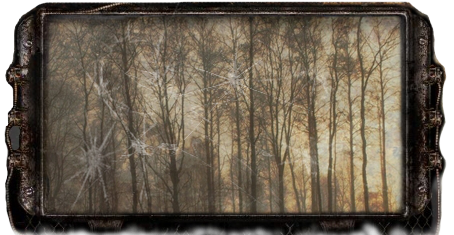
\includegraphics[width=.6\hsize, clip = true, trim = 0 0 0 0]{ro4_pietno.png}
\end{figure}
% 
Las w ujęciu zmysłów emanował nieokreśloną energią, ledwie wyczuwalną, ale poruszającą sferę ludzkiej psychiki. Dumnie szumiące ramiona drzew nękane przez powiew wiatru symultanicznie ociekały rześkimi kroplami deszczu. Wolno spijana przez glebę woda tworzyła cieniutkie strużki na kolorowych liściach, chlapiąc tym samym małych mieszkańców ściółki. Powietrze przesycone wilgocią czyniło to miejsce bardzo zmysłowym, wzruszona leśna ziemia mieszała w sobie kolory połyskując w świetle rzucanym za przyzwoleniem gęstych gałęzi. Ceremonię natury kształtował harmonijny wokal ptasiego klanu. Duch lasu oswoił się z nowym przybyszem, pozwolił mu na pobyt w królestwie dziewiczej biosfery. Obcy odziany w płaszcz wkroczył do świata, gdzie człowiek jest intruzem zdanym na łaskę przyrody, miejsca, gdzie wołanie o pomoc jest zjawiskiem próżnym, a każdy kolejny krok to próba. Z perspektywy naukowca czarujący bezlik dziewiczej krainy, na mapie malutki nic nieznaczący punkcik. 

Giennadij krocząc po miękkim gruncie świdrował wzrokiem strzeliste sosny oraz wsłuchiwał się melodyczną fonię niesioną przez oddech lasu. Licznik Geigera milczał pozwalając poruszać się w równym tempie, chód zakłócały tylko bujne krzewy o długich haczących gałązkach. Bór należał do Strefy jednak znajdował się znacznie dalej od centrum wydarzeń z pamiętnego 1986 roku. Wszakże sam fakt przynależności lasu do regionu wokół Czarnobyla wyraźnie zniechęcał ludzi do zapuszczania się na te tereny. Giennadij z każdym kolejnym krokiem oddalał się od pozostawionego samochodu, naturalne bariery w formie gęstej roślinności wyrastały proporcjonalnie do przebytej drogi. Walka z gąszczem była wycieńczająca, im dalej szedł tym krzaczaste zarośla coraz mocniej utrudniały posuwanie się naprzód. Taki stan rzeczy wysuwał przypuszczenia na temat ostatnich wizyt człowieka w tym miejscu, naukowiec do tej pory nie dostrzegł niczego co mogło, by pochodzić od ludzi, żadnych śmieci czy wydeptanych ścieżek. Katastrofa, choć wyrządziła wiele szkód i cierpienia mieszkańcom Czarnobyla to dla lasu okazała się zbawienna. 

Giennadij nadal toczył uciążliwe zmagania z krzewami odgradzając przejście poharatanymi dłoniami. Mozolne przedzieranie się przerwał sygnał telefonu. Naukowiec wzdrygnął i w okamgnieniu odebrał połączenie. Po przeciwnej stronie odezwał się znajomy głos: 

-- Giennadij, gdzie ty u licha jesteś! Powinieneś już dawny być w pracy, stało się coś? -- cedził zdenerwowany Wuser. 
-- Słuchaj mnie uważnie\3kW drodze do Prypeci zauważyłem coś, co przypominało ludzką istotę! Cholera wie\3k 
-- Jaja se robisz, gdzie ty ku*wa jesteś? 
-- W jednym z lasów, kilka kilometrów od Korogodu, kieruj się w te strony, na poboczu stoi mój samochód, będę przy, nim czekał. 
-- Zachciało ci się w detektywa bawić. Radzę ci ulotnij się stamtąd jak najszybciej, bo nie wiesz z czym masz do czynienia. Spróbuję cię usprawiedliwić w kierownictwie i zaraz ruszam! 

Głos dobiegający ze słuchawki zamilkł. Giennadij zdał sobie sprawę, że impulsywne podjęcie śledztwa wymazało jakiekolwiek oznaki trzeźwego myślenia. Poczuł na sobie ciężar chwili, sytuacja w jakiej się znalazł była dość skomplikowana --on sam w centrum dziczy jako poszukiwacz niezidentyfikowanej formy życia. Krople potu ciekły mu po skroniach, cierpki smak strachu objawił się paraliżującym ciało na wskroś uczuciem gęsiej skórki. Efemeryczne poruszenie tchnęło w naukowca nowe siły uwalniając go ze stagnacji. Giennadij obrócił się na pięcie i zaczął zmierzać w kierunku wyjścia. Las w perspektywie czasu stracił swój dawny urok, niewidzialne napięcie nadgryzało świadomość bohatera trując jego psychikę nienamacalną energią grozy. Mózg poddając się nieprzyjemnej woli lęku płatał figle kreując coraz to bardziej pokręcone obrazy. Towarzyszący niepokój narastał, otaczający go obszar wznosił niemal celowy opór. Każdy ruch bohatera zdawał się być kontrolowany przez siły wyższe, a wszelkie próby przełamania nieuchwytnych barier ponosiły fiasko. Giennadij czuł jak ziemia pod, nim mięknie, a nogi twardnieją. Przytłumiony natłokiem nadprzyrodzonych zdarzeń naukowiec machinalnie sięgnął do kieszeni. Wskazówki kieszonkowego zegarka stanęły w miejscu. Bohater uparcie parł na przód potykając się o wystające z ziemi korzenie. Momentalnie w uszach rozległ się rozdzierający pisk, a w głowie powstała absolutna próżnia. Giennadij upadł na kolana. Spazmatycznie skierował wzrok przed siebie rozwierając usta i mamrocząc coś pod nosem. Dusza bohatera zdawała się odrywać od ciała, by pożegnać sferę materialną i rozpłynąć się gdzieś w świecie astralnym. 

Śmierć zamiast spojrzeć ostatni raz w oczy pozwoliła zobaczyć to czego tak bardzo szukał. Za drzewami rysowała się sylwetka humanoida o dziwacznej posturze. Zagadkowa istota ospale kroczyła w kierunku będącego w transie Giennadija. Dystans dzielący obie postacie pozwalał wyłącznie na kontakt wzrokowy. W pewnej chwili enigmatyczny mieszkaniec lasu znieruchomiał nieprzerwanie wpatrując się w naukowca. Ten zaś ostatnie resztki sił skupił na wymianie chaotycznych spojrzeń z potencjalnym przeciwnikiem. Kres życia zdawał się być nieunikniony, cena maniakalnego dążenia do poznania prawdy okazała się zgubna. Bohater poczuł w piersi ścisk, cząsteczkę żalu jak cierń raniącą duszę przegranego. Bezimienny twór uniósł rękę przed siebie wymierzając finalny wyrok. Pisk ponownie przeszył przestrzeń zwiastując nieubłagany koniec. Niespotykana dotąd atmosfera grozy pękła niczym bańka, zmyła się pozostawiając po sobie tylko wspomnienie. Umysłowa katorga dobiegła końca przejaśniając rzeczywisty obraz. Giennadij czuł przyrost wigoru. Nie odrywał jednak wzroku od wciąż będącej naprzeciw postaci. Obcy opuścił kończynę spojrzał ostatni raz i rozpłynął się w gęstwinie lasu. 

Bohater wstał nie okazując żadnych oznak wycieńczenia, poczuł się, jak, gdyby nic się nie stało. Świadomość psychicznej konfrontacji wciąż tliła się w środku szukając racjonalnego wytłumaczenia. Giennadij nie zadawał już pytań, chciał uchwycić sens, poznać odpowiedź. Mechanizm kieszonkowego zegarka funkcjonował bez ustanku cyklicznie przesuwając wskazówki. Naukowiec wskrzesił pamięć 
i uzmysłowił sobie, że w jego stronę zmierza Wuser. Otrząsnął się ostatni raz i żwawo podążył ku drodze powrotnej. Samochód stał na poboczu połyskując w blasku słońca. Giennadij usiadł na masce i wyczekiwał przyjazdu znajomego. Z oddali dochodził dźwięk pracującego silnika, niebawem na asfaltowym płótnie pojawiły się kontury pędzącego pojazdu. Czterokołowa maszyna zatrzymała się tuż obok naukowca. Wuser wybuchowo wysiadł i przemówił gubiąc dech: 
--Giennadij niech cię szlag trafi. W co ty pogrywasz, życie ci nie miłe, co widziałeś, opowiadaj! 
--Skąd mam wiedzieć. Kosmitę? Istotę o dość dziwnej głowie i posturze. Nie miałem okazji zobaczyć go z bliska, ale\3k -- naukowiec urwał. 
--Co ale? 
--Zdolności paranormalne\3k 
--Pieprzysz głupoty. Może chcesz mi wmówić, że unosił się w powietrzu, a następnie wyciągnął królika z kapelusza. Nie żartuj! -- znajomy zrobił pogardliwą minę i wlepił wzrok w zmieszanego Giennadija. 
--Wuser to, co doświadczyłem nie można zilustrować w realny sposób, to było coś jak przejście na tamten drugi świat. 
--Rozmawiałeś z Bogiem? 
--Choć za mną niedowiarku, poszukamy razem tej tajemniczej istoty -- rzucił z powagą i ruszył w stronę lasu. 
--Prowadź -- odrzekł lakonicznie, wsadził ręce do kieszeni i udał się za kolegą. 
Po pokonaniu kilku metrów Giennadij zachwiał się i spłynął na ziemie podpierając się w ostatniej chwili rękoma. Świat ponownie zawirował. Powieki stały się ciężkie, naukowiec z trudem obrócił głowę. Niewyraźny profil człowieka spoglądał w bezruchu na tracącego kontakt z rzeczywistością Giennadija. Konający zdołał wykrztusić ostatnie słowa. 
--On\3ktuu jest\3k 
--Ja tu jestem, wybacz stary\3k 
Wuser rzucił na ziemię zużytą strzykawkę z nieznanym środkiem. Podniósł leżącego i zaprowadził do pojazdu. Chwilę potem na poboczu pozostał już tylko jeden samochód.


Rozdział V
Droga:  

W małym pomieszczeniu obitym mlecznymi kafelkami unosił się wyraźny zapach laboratoryjnego sprzętu. Nieskazitelnie czysta podłoga oślepiająco połyskiwała za sprawą intensywnie świecących jarzeniówek. Szczelnie zamknięte drzwi torowały zgiełk dobiegający z korytarzy pozwalając tylko nielicznym dźwiękom, choć stłumionym dotrzeć do pokoju. Na środku salki znajdował się kredens z różnorodnymi instrumentami i środkami medycznymi, w rogu zaś usadowiono potężną szafę z rzeczami o nieznanej wartości. Na tarczy ściennego czasomierzu wskazówki manifestowały godzinę trzynastą. 
-- Sądzi pan, że ten zabieg zakończy się pomyślnie, operacja nie może ponieść za sobą żadnych konsekwencji. Prawda nie może wyjść na jaw -- zakomunikował jeden z ludzi znajdujących się w pomieszczeniu. 
-- Absolutnie. Proszę mi zaufać. Znam się na tym -- Wuser wstał naciągnął strzykawkę i dodał -- podjęcie takich działań wymagało obejścia wielu przeszkód, tym samym wykorzystałem limit przywilejów w kierownictwie. Dobrze, że o niczym nie wiedzą. 
Cieniutka igła bez oporu wbiła się pod skórę nieprzytomnego mężczyzny wprowadzając preparat do organizmu. W tym samym czasie z drugiego końca sali dobiegł tubalny głos kolejnego gościa: 
-- Jak długo mamy czekać i pytanie co dalej? 
-- Preparat zacznie funkcjonować w granicach pięciu minut. W tym czasie warto obmyślić alternatywną wersję zdarzeń i przedstawić ja Giennadijowi -- oznajmił Wuser wrzucając do kosza zużyty iniektor. 
-- Ja z, nim porozmawiam -- wymamrotał mężczyzna teatralnie poprawiając krawat -- następnie przedstawimy po kolei etapy jego nowej pracy. 
-- Kontaktowałem się z Kaługinem w dzisiejszej sprawie, nie ukrywał zaniepokojenia -- stwierdził jeden przyglądając się nieprzytomnemu. 
-- Akurat Kaługin, to nasze najmniejsze zmartwienie. Za jakiś czas dowiemy się, na czym dokładnie stoimy. O wybudza się! -- ożywił się facet w garniturze podchodząc do Giennadija. 
Zgromadzeni zebrali się obok wracającego do rzeczywistości naukowca w zaciekawieniu obserwując jego mimowolne tiki i pomrukiwania. Półprzytomny niemrawie unosił powieki, łzawiąc z powodu mocnego światła. Naukowiec gwałtownie się poruszył, spuszczając głowę, mamrotał pod nosem, ogarniając wzrokiem niewyraźny obraz. 

Niedobudzony, ale kontaktujący mniej więcej spojrzał na trzech facetów w garniturze, jednego z nich, choć rozmazanego rozpoznał od razu. Giennadij złapał się za głowę i rzekł standardowo: 
--W mordę, moja głowa. Co ja tu robię 
--Witaj Gienna, widzę dochodzisz do siebie, lek zaczyna działać -- rzucił Wuser na przywitanie. 
--Jaki lek, co tu się dzieję, gdzie ja jestem? -- pytał podenerwowany naukowiec domagając się odpowiedzi. 
--Proszę być spokojnym. Wszystko jest pod kontrolą, postaram się panu wszystko wyjaśnić. Nazywam się Matwiej Gusiniew, a to mój towarzysz Nikołaj Wawiłow, mamy zamiar nakreślić kilka spraw odnośnie stażu. Ale najpierw wyklaruje sytuacje, która pana niecierpliwi. Giennadij, podczas kierowania się w stronę Prypeci prawdopodobnie zemdlałeś, jako nieprzytomny zostałeś przetransportowany właśnie tutaj. Nie znamy na razie przyczyn tego niefortunnego zdarzenia, całe szczęście jest pan z nami cały i zdrowy. Wszystko dzięki Wuserowi, który udzielił pomocy. Ale do rzeczy, udamy się zaraz do pokoju, gdzie podpisze pan jeszcze kilka papierów i następnie skierujemy się w stronę Czarnobyla, gdzie mieści się nasza placówka. Proszę za mną. -- Gusiniew podniósł teczkę, wręczył poszkodowanemu osobiste rzeczy i dłonią wskazał drzwi wyjściowe. 
--Pozwólcie, że udam się do łazienki. To potrwa chwilę -- powiedział Giennadij opuszczając trójkę mężczyzn. 
Trzech facetów wyszło na zewnątrz i zaczęło rozmawiać, echo wypowiadanych słów niosło się długim korytarzem rozpływając się i pozostawiając po sobie tylko wątły pomruk. Giennadij oparł się o umywalkę przemywając twarz letnią wodą, nieco orzeźwiony zerknął w lustro dostrzegając dziwne znamię w oku. Naukowiec przyjrzał się bliżej, czarna plamka na twardówce, choć mała była dobrze widoczna. Giennadij nieco zaniepokojony wciąż przyglądał się w zwierciadle, usiłując wytłumaczyć pochodzenie nieproszonego gościa. Do łazienki raptownie wtargnął Wuser poganiając naukowca, ten szybko się zerwał zakrywając dłonią oko udając, że je przemywa. 
-- Co ty makijaż robisz? Nie ma czasu, trzeba ruszać -- stanowczo, choć bez irytacji pośpieszył kolegę. 
Przed budynkiem stał już samochód, elegancka limuzyna z otwartymi drzwiami czekała, by zabrać pasażerów do Czarnobyla. Brodaty szofer w swetrze i jasnych dżinsach dopalał właśnie papierosa, gdy czterech mężczyzn wsiadało do auta. Gusiniew ponaglił kierowcę i po chwili maszyna na kołach chwiejnie z impetem wyjechała z placówki kompleksu badawczego. 

Pojazd sunął po szosie mijając co rusz porośnięte bluszczem domki i znaki informujące o skażeniu radioaktywnym. Upiorne budynki bez okien i drzwi wyrastały ponad widnokrąg, a w bujnych trawach topiły się zdezelowane przedmioty i przerdzewiałe wraki pojazdów. Miejsce zapomniane, wyobcowane, nasiąknięte pustką i chłodem. Grobowy krajobraz stworzony i zniszczony przez ludzi.
Po długim milczeniu w samochodzie rozległ się tubalny głos Wawiłowa: 
-- Jeszcze jakieś z dziesięć minut, zaraz wjedziemy na most śmierci. 
-- Skąd taka nazwa, mogę się domyślać? -- rzucił pytająco Giennadij 
-- Podczas katastrofy mieszkańcy zgromadzili się na moście, by obserwować skutki wybuchu reaktora. Rzekomo wszyscy ci, którzy w tym dniu stali na wiadukcie zmarli po jakimś czasie. Teren był bombardowany przez większe ilości promieniowania, oczywiście nie wiadomo czy historia jest prawdziwa, ale nazwa jak widać przetrwała. 
-- Ciekawa anegdota -- odpowiedział naukowiec i ponownie wlepił wzrok w szybę. 
-- Spójrzcie w lewo, dzik przy drodze\3kCałkiem spore -- oznajmił Wuser ożywiając nieco panującą atmosferę. 
-- Normalka, codziennie takie widzę. Wyrośnięte, to takie\3kAle można by wyżywić cały personel przynajmniej -- odrzekł ponownie Wawiłow sztachając się fajką -- o już dojeżdżamy. 

Z mostu doskonale widać było charakterystyczny komin reaktora, na wysokości wzniesienia górowały korony drzew oraz, ledwo widzialne szkielety budynków. Niebo formowały kłębiaste chmury o ponurej barwie, te niesione wiatrem przemieszczały się na tle statycznej konstrukcji -- symbolu katastrofy energetyki jądrowej. 
Limuzyna zjechała z głównej szosy jednocześnie tracąc z pola widzenia prospekt martwego miasta. Samochód zbliżał się do posterunku, przy, którym stało kilku uzbrojonych mężczyzn. Szofer zasygnalizował za pomocą świateł, że zbliża się jednostka urzędowa. Pięć mrugnięć wystarczyło, by paru rosłych facetów gwałtownie uniosło szlaban. Pokonanie bariery przeszło bezproblemowo, jednak tym razem postój był konieczny. Przy następnym posterunku zaczęto legitymować pasażerów, mimo wysoko postawionych członków tajnego kompleksu. Pragmatyczne metody działania obejmowały każdego. Strażnicy zasalutowali na odczepnego i wrócili do swoich spraw, przed samochodem rysował się krótki odcinek drogi, który urywał się w pewnym miejscu. Po prawej stronie zaczynał się brukowany chodnik otoczony siatką i podejrzanymi prętami wystającymi z ziemi. 
-- To tutaj. Wysiadamy -- odparł Wawiłow 
-- Spodziewałem się czegoś innego, poza chodnikiem i ogrodzeniem nie widzę tu niczego co mogło, by służyć za ośrodek badań -- rzucił z lekką ironią Giennadij spoglądając na mężczyzn. 
-- Jeszcze nie dotarliśmy do celu, niech pan się nie martwi. Proszę za mną. 
Gusiniew pozdrowił szofera i limuzyna odjechała. 
-- Nie muszę przypominać, że przedsięwzięcie, w którym bierze pan udział jest tajne. Tak, więc wyjaśnię jeszcze kilka kwestii -- Gusiniew zrobił pauzę zerknął na naukowca i dodał -- cały kompleks mieści się pod ziemią. Badania jakie prowadzimy są nad wyraz cenne i niebezpieczne, z tego powodu byliśmy zmuszeni kierować całą akcją z dala od osób postronnych, czy też wścibskiego wywiadu krajów zagranicznych. Zwierzchnikiem projektu jest Kaługin, myślę, że zdoła go pan jeszcze dzisiaj poznać.

Panowie skręcili w jedno z odgałęzień i znaleźli się na przeciw małego budyneczku o wojskowym charakterze. Betonowa konstrukcja wyrastała z ziemi pod kątem ostrym. Stalowe wrota zgrzytnęły, a blade światło padło na schody prowadzące pod ziemię. Przed drzwiami stał funkcjonariusz z karabinem zawieszonym na plecach, ten przed oddelegowaniem otrzymał jakieś instrukcje od Gusiniewa, anonimowy pracownik obrzucił wzrokiem na gości i zaprosił do środka. Giennadij przed wejściem spojrzał jeszcze raz na zegarek, niebawem potężna brama za jego plecami zadudniła wydobywając z siebie głuche szczęknięcie.



Rozdział VI
Pokój numer 12:  

Image

Żelbetowa konstrukcja nad głowami czterech mężczyzn przytłaczała kształtem i wysokością. Niski sufit sprawiał, że miejsce budziło dyskomfort i poczucie stąpania pod powierzchnią, pomimo że panowie niezeszli jeszcze pod umowny poziom morza. Stalowe linie biegnące wzdłuż pomieszczenia skrywały pod powłoką przewody elektryczne, które gdzieniegdzie rozwidlały się i wtapiały w masywne betonowe mury. Sklepienie skromnie urządzono nagimi żarówkami, od, których biło słabe pulsujące światło, co kilka metrów z krawędzi ścian wyłaniały się ziejące czernią otwory, służące za kanały wentylacyjny. Korytarz w pewnym miejscu się kończył, a Giennadij wraz z tajemniczą kliką był zmuszony poczekać, aż z malutkiego pokoiku wygramoli się strażnik z pękiem kluczy. Pełniący wartę pracownik zająknął coś pod nosem, że tylko on wiedział co ma na myśli. Wątły łysiejący facet w okularach z lat siedemdziesiątych i dziwnym zaczesem na głowie sprawiał wrażenie człowieka egzystującego wyłącznie w tej betonowej jaskini, w której zatrzymał się czas. Giennadij spoglądał na otwierającego drzwi mężczyznę, choć bardziej interesował go zamknięty tuż obok pokój z symbolem H--3. Przez wizjer naukowiec ujrzał zniekształcony i nic nieznaczący obraz, aczkolwiek stale zmieniający się. 

-- Do jakich celów asygnowany został ten pokój? 
-- Nie możemy obecnie udzielić informacji na ten temat. Wybaczy pan. 
Po tych słowach portier zerknął na dociekliwego naukowca, lekko zatroskana mina zdradzała jakieś wewnętrzne zaniepokojenie, po chwili woźny spojrzeniem ogarniał już tylko kiść mosiężnych kluczy. Hermetyczne wrota zgrzytnęły donośnie, masywne skrzydło przesunęło się w bok wpuszczając do pomieszczenia dawkę rażącego światła. Mężczyźni bez wahania ruszyli, skinęli rękoma w podzięce i w milczeniu podążyli w kierunku kolejnych drzwi, przy, których czekał wcześniej poinformowany nadzorca. 
-- Dzień dobry, poproszę klucz do holu nr 4. 
Gusiniew surowo zakomunikował i podkreślił swoje żądania, strażnik lekko wzdrygnął i wykonał polecenie. Dla Giennadija wydawał się to ostatni etap zwiedzania tajnego kompleksu, jednak rysujący się przed jego oczyma widok kolejnych korytarzy i drzwi rozwiał osobiste dywagacje wywołując zarazem zażenowanie i ospałość. 

-- Proszę tutaj, lada moment będziemy na miejscu -- Nikołaj zachęcająco wskazał ręką na przejście po ich prawej stronie, gdy wszyscy znaleźli się w małym przedsionku wezwano windę za pośrednictwem kodu. Parę kliknięć w panel sterowania sprawiło, że serce maszynerii wróciło do życia, zespół różnorodnych elementów zaczął współgrać ze sobą jak orkiestra podczas koncertu, wydając przy tym mechaniczną kakofonię, która narastała z każdą sekundą. Dźwignik podążał ku górze, stalowa nić za niewielką witryną wyglądała dość upiornie, jak wąż, który utknął w ciemnościach i wije się w otchłani. Na finiszu winda wydała charakterystyczny brzęk, blokada przestała spełniać swą funkcje i zgromadzeni mogli zjechać na niższe kondygnacje. Mężczyźni w ciągu niecałej minuty znaleźli się kilkadziesiąt metrów pod ziemią, gdy drzwi odsunęły się na bok Giennadij momentalnie się ożywił. Przestrzeń, choć nie różniła się rozmiarem od poprzednich miejsc, uderzała niezwykłą dbałością i znamienną elegancją, przejrzysty wykafelkowany korytarz bił po oczach przyzwyczajonych do smętnego światła. Lokum tętniło życiem, echo kroków chodzących pracowników rozchodziło się ze znaczną częstotliwością, tu i ówdzie rozbrzmiewały dźwięki wydawane przez laboratoryjną aparaturę. Cały personel posiadał jednolity ubiór, biały kombinezon z maseczką, solidne buty kształtem przypominające gumiaki i podręczny notes. Naukowcy pochłonięci pracą nie zwracali uwagi na gości, przechodzili obok przybyszów nie odzywając się ani słowem. nawet do wyżej ustawionych Gusiniewa i Wawiłowa. 
-- Zapraszam wszystkich do pokoju, odpoczniemy chwilę i przejdziemy do konkretów. Giennadij, za jakiś czas powinieneś otrzymać klucze oraz instrukcje, które pozwolą ci się oswoić z nowym otoczeniem, resztę ludzi poznasz jutro. Kawy? -- Wawiłow załączył elektryczny czajnik i przysiadł do stołu. 

Giennadij z aprobatą przyjął poczęstunek, gdy miał zadać kilka pytań dotyczących stanowiska, kątem oka dostrzegł pracownika niosącego w ręce coś na podobieństwo kajdanek. Lekko zdumiony naukowiec szukał wytłumaczenia, w jakim celu zostały przyniesione owe bransolety. Ostatecznie Giennadij wstrzymał się z reakcją i oponował swoją dociekliwość. Z naczynia zaczęła buchać para i w mgnieniu oka kubek przepełnił się wrzącym naparem. W pomieszczeniu zapanowała usypiająca aura, jednak dość przyjemna w odbiorze, miękkie obicia krzeseł zapewniały komfort i poniekąd stały się powodem, dla którego zgromadzeni rozpłynęli się w objęciach drewnianych siedzeń przy okazji racząc się zapachem czarnego wywaru. Nie długo trwała ta cisza, do pokoju wtargnął nieznajomy mężczyzna ubrany w biały kombinezon. Zdjął maskę ochronną, z jego czoła zaczęły spływać krople potu, zgrzany facet dłonią przeczesał grzywę do tyłu i uśmiechnął się do wszystkich.
-- Nazywam się Matwiej Akwajip, a pan jak dobrze myślę, Giennadij -- żywiołowy pracownik kompleksu wyciągnął z kieszeni jakieś drobiazgi, wśród nich był kluczyk z breloczkiem informującym do jakich drzwi pasuje. Na metalowej blaszce widniała naklejona liczba -- 12. Naukowiec z racji respektowania manier wstał i przywitał się przytakując głową na wcześniejsze pytanie. 
-- Pozwoli pan, że się streszczę. Udamy się teraz do innego miejsca, tam wytłumaczę pokrótce co i jak. To w drogę. Do widzenia wszystkim -- Matwiej energicznie uściskał dłonie pozostałym i wyszedł z pokoju. Giennadij zrobił to samo. Wawiłow, Gusiniew oraz Wuser także opuścili lokum, obierając zupełnie inną trasę. 
-- Otrzyma pan drugi klucz do "dwunastki", obecnie w laboratorium tylko dwie osoby mają dostęp do tego pomieszczenia. Kombinezon czeka już w szatni, a niezbędne przyrządy przekażę już na miejscu. Od razu przejdę do meritum, w sali dwanaście, dwunastce, jeden dwa, szczurowni czy jak, kto woli prowadzimy eksperymenty na zwierzętach, łatwo domniemać na jakich. Od razu przestrzegam, że te małe ścierwa są dość agresywne i trzeba mieć co nie co animuszu przy obcowaniu z tymi stworzonkami. Niektóre okazy są wyrośnięte, ale jak je porządnie pacnąć to się uspakajają, badamy ich psychikę, tresujemy i inne takie, resztę szczegółów pozna pan z czasem. O! Tutaj jest przebieralnia -- Matwiej uchylił drzwi od szatni i pożegnał się z Giennadijem na kilka minut. 

Naukowiec spojrzał na żwawego pracownika wertującego po drodze kartki podręcznego notesu. Po chwili znikł mu z oczu, a korytarz oblała pustka, blade ściany, choć biły światłem spowiły powietrze zdechłą aurą, wszystko ucichło. Laboratoryjny zgiełk przeistoczył się w próg słyszalności, podziemny kompleks wydawał się być martwy. Giennadij otworzył drzwi na oścież, rząd metalowych szafek rozpościerał się na pół sali, tu również nikogo nie było, tylko zdeformowana postać żyjąca w lustrzanym świecie na płaszczyźnie stalowego prostopadłościanu. Na ławie znajdował się poskładany kombinezon, obok masywne gumofilce wyglądające jakby przed chwilą opuściły taśmę produkcyjną. Naukowiec wskoczył w biały kostium, dopiął guziki w rękawach i machinalnie poprawił nogawki, obuty jak należy mógł pełnoprawnie stać się członkiem personelu. Do kieszeni wrzucił zegarek, jednak po chwili wyciągnął go z powrotem. Wskazówki nie przemieszczały się, sekundnik żałośnie dogorywał próbując przemieszczać się ku górze, na tarczy chronometru czas stanął w miejscu. Do szatni napłynął strumień światła i dźwięk kroków. Uśmiechnięty Matwiej stanął w progu i rzucił: 

--Widzę, że jesteś już gotowy, w takim razie zapraszam. Potrzeba czegoś jeszcze? 
--Baterii. Mój zegarek przestał działać. -- odparł Giennadij stukając palcem w szybkę wartościowej pamiątki. 
--Znajdzie się, jednak teraz proszę za mną. 
Pokój numer dwanaście mieścił się na końcu holu, obok niego znajdował się również gabinet o nieznanym przeznaczeniu. Zawieszona tabliczka informowała o jakimś niebezpieczeństwie, lecz naukowiec nie przyjrzał się dostatecznie, by zrozumieć jej graficzne obwieszczenie. Akwajip włożył klucz do zamka, zespół drobnych zapadek przyjął prawidłową kombinację, wrota otwarły się. W pomieszczeniu było ciemniej niż na korytarzu, źródłem światła okazały się zwykłe lampki stołowe rozmieszczone według przyjętego schematu. Na środku stały żelazne bryły wyposażone w liczne pokrętła, suwaki oraz liczniki. Na biurkach usytuowane były komputery starego typu, podłoga była tutaj brudna, a powietrzu unosił się swąd futra i fekaliów. 
-- Proszę założyć maskę, chyba że odpowiada panu ten zapaszek -- Matwiej zaśmiał się pod nosem. 
-- Nie tak sobie to wyobrażałem. Myślałem, że\3k 
-- Że co? Że to będzie salon gier, ze szwedzkim stołem i półnagimi panienkami na parkiecie? -- Akwajip znów buchnął śmiechem, jednak zrobił to na tyle uprzejmie , że sam Giennadij zachichotał. 
-- Gdy tu trafiłem też się zniesmaczyłem, ale przyzwyczaiłem się i wiesz co? Polubiłem tę robotę, tobie też się wkręci. Choć pokaże Ci moje pociechy -- Matwiej wyciągnął z kieszeni ostry przedmiot i zniknął za aparaturą. 
Szczury przebywały w odosobnionych klatkach, obserwacja zwierząt odbywała się przez specjalne wizjery wbudowane w stalowe drzwiczki. Dodatkowo każdy zasobnik wyekwipowany był w dwa otwory, przez, które podawano substancje. 

-- Tego nazwałem Lozo, jest tu najdłużej ze wszystkich, najbardziej posłuszny i najbardziej zmutowany. Powinien już dawno nie żyć, ale jak widać katastrofa okazała miłosierdzie tym ssakom. Lozo nie posiada oczu, w sumie to posiada, ale to tylko taki dodatek, zmysł wzroku całkowicie u niego zanikł jak u reszty. Mimo, to jest wrażliwy na światło i przedmioty wytwarzające zmienne pole elektromagnetyczne. Niech sobie pan wyobrazi, że wypuszczamy je z klatki, pozbawiamy węchu oraz słuchu, my zaś stajemy w umownym bezruchu gdzieś na końcu ciemnego pomieszczenia, szczury bez problemu nas znajdą. Impulsy elektryczne wytwarzane przez skurcze naszych mięśni zdradziłyby nasze położenie, nie wiemy tylko jaki organ u tych zwierząt spełnia rolę elektroreceptora. Jak dotąd jedynymi ssakami posiadającymi tę zdolność były dziobaki oraz delfiny rodzaju sotalia. Proszę spojrzeć, obok Lozo leży przedmiot, który za moim pośrednictwem otrzyma ładunek elektryczny. 
Matwiej wykonał serię nieskomplikowanych ruchów dłonią na tablicy urządzenia sterującego. Zielona dioda zasygnalizowała przepływ prądu, szczur w oka mgnieniu zerwał się i skierował w stronę tajemniczego przedmiotu. Lozo zaczął obwąchiwać obiekt, ale szybko się znudził i wrócił do leżenia. 
-- Teza o wytworzeniu zmysłu elektrolokacji u szczurów wydaje się być jak najbardziej prawdziwa. Wystarczy sporządzić wnikliwy raport. 
-- I ja go mam stworzyć? -- odezwał się Giennadij po dłuższej przerwie. 
-- Nie , nie. To moja działka. Pan będzie miał inne zadanie. Prowadzimy również eksperymenty nad świadomością tych ssaków, posiadamy specjalny emiter generujący promieniowanie o niskiej częstotliwości. Chcemy wpływać na zachowanie szczurów. Aktualnie wyniki pomiarów są skąpe, ale w przyszłości ma się to zmienić. 
-- Nie sądziłem, że zakres doświadczeń obejmują tak złożone technologicznie metody. Brzmi ciekawie. 
-- W zeszłym tygodniu doszło do pierwszej próby, w której dwa egzemplarze zostały potraktowane sporą dawką radiacji. Nie mamy jeszcze przyjętej nazwy dla tego rodzaju promieniowania, ale wiemy jak je uzyskiwać. To bardzo skomplikowana procedura. Proszę za mną. 

Akwajip otworzył klatkę, opryskał szczura płynem najwidoczniej powodującym zmniejszenie agresji. Złapał otępiałego futrzaka w rękawice i przeniósł do enigmatycznej maszyny, która Giennadijowi nie rzuciła się wcześniej w oczy. Agregat miał symetryczny układ, po obu stronach widniały silosy wypełnione żółtą cieszą. Na środku znajdował się piedestał otoczony do połowy miedzianą cewką, z górnej powierzchni okrągłego modułu wystawał bolec z kulistym zakończeniem. Maszyna zawyła, bęben obrócił się o dziewięćdziesiąt stopni umożliwiając Matwiejowi ulokowanie bezwładnego szczura. Aparatura pracowała na jałowym biegu. Naukowiec podał zwierzęciu miksturę za pomocą zastrzyku i oddalił się od urządzenia. Obaj panowie stali przy sterowni osłoniętej ołowiową szybą. Chwilę potem antena stanowiąca wierzch maszyny wykrzesała z siebie iskry i okryła się elektryczną nicią. Cewka zaczęła się powoli obracać, nad szczurem rozbłysło łagodne światło. Proces radiacji bezbronnego stworzenia odbywał się bez szwanku, mikroskopijny świat nad ciałem gryzonia szalał jak burza, masa cząsteczek z szaleńczą prędkością odbijała się od siebie w nieskończoność, swoista entropia dobiegła kresu, gdy Matwiej wyłączył mechanizm startowy. 
-- Pierwszy etap zakończony pomyślnie, musimy odczekać kwadrans, aż nasz mały przyjaciel wróci do świata żywych. 
Naukowiec przysiadł do biurka i zaczął studiować zapiski na ekranie monitora. Giennadij tylko się przyglądał i czekał na swoją kolej. W międzyczasie zerknął na zegarek, wskazówka wyznaczająca sekundy jak, gdyby nigdy nic zmierzała ku górze zataczając wieczny okrąg.


Rozdział VII
Widmo:  

Napięta twarz naukowca mieniła się na niebiesko. Matwiej pochłaniał spojrzeniem wyświetlany na ekranie wykaz zakończonego badania, diagramy okraszone skomplikowaną symboliką owocowały u niego napięciem, urzeczywistniającym się w postaci mimowolnego pomrukiwania i mrużenia oczu. Giennadij wyłapywał sens poszczególnych linijek, ale nie mógł dokładnie stwierdzić istoty graficznych znaków. 
-- Niech pan spojrzy tutaj, na ten wykres -- Akwajip zaczął jeździć palcem po ekranie -- komórki mózgu odpowiedzialne za świadomość są tak jakby wyłączone. Szczur żyje, ale nic nie może robić. Możemy teraz ingerować w jego umysł, oddziałując cząsteczkami pobudzającymi niepracujący obecnie organ. Każdy z okazów ma wszczepiony chip, który jest czymś w rodzaju łącznika odbierającego informacje wysyłane przez nas i dalej do mózgu. Niezwykłe. Eksperymenty nie zawsze się sprawdzały, ale kilka prób dały nam punkt odniesienia i wiemy, na czym stoimy. Kontrola świadomości to ogromny krok na przód, ale za nim opatentujemy w stu procentach ten wieloaspektowy proces minie dużo czasu. 
-- W swoich badaniach zajmowałem się głównie oddziaływaniem promieniowania na roślinność. Nie sądziłem, że poznawanie strefy może się odbywać na inne sposoby -- Giennadij skrzyżował ręce, pochylił się nad monitorem i odrzekł -- A czy szczury są tu jedynym rekwizytem doświadczalnym? 
-- Nie. Ale zakres naszych możliwości rozwinął się do takiego stopnia, żeby brać pod uwagę inne gatunki zwierząt -- Matwiej odszedł od komputera niknąc w mroku. 
-- Rozumiem. 
Giennadij przez moment stał sam w wydzielonym pomieszczeniu i świdrował wzrokiem znajdujące się wokół konsolety. Wówczas z końca pokoju dobiegł niekształtny głos naukowca. 
-- Trochę tu razem przepracujemy, co pan powie na wypad do pobliskiego bufetu po zakończeniu pracy? Serwują tam również alkohol, ale za specjalnym przyzwoleniem. 
-- Kilka głębszych nie zaszkodzi -- odparł, wypatrując z ciemności sylwetkę Matwieja. 
-- Szybko pan podjął decyzję o zmianie stanowiska, nie podobało się w Prypeci? 
-- Dziwnie to zabrzmi, ale trochę tęsknie za swoim gabinetem, ten sam widok przez pięć lat. Człowiek przyzwyczaja się do pewnych miejsc. Za namową Wusera zmieniłem funkcję, dość pochopnie\3kZ natury jestem ciekawski i lubię poszerzać horyzonty. Sądzę, że dobrze zrobiłem. 
-- Dobrze pan sądzi, Wuser pracuje tu od dłuższego czasu. Nie za często się z nim widuje, ale równy gość z niego. Nie wspominał wcześniej o tym laboratorium? 
-- Właśnie się zastanawiam, czemu milczał skubany i jakim cudem dzielił etaty, skoro widywałem go w Prypeci. Czyżby tajemnica zawodowa? 
-- Słusznie. Warunki są dość rygorystyczne, poza terenem kompleksu nie warto sobie robić problemów, ściany mają uszy, a może cała strefa to jeden wielki podsłuch? -- Matwiej uśmiechnął się i zdjął rękawice ochronne -- Czas na przerwę. 
Obydwaj ruszyli w stronę wyjścia. Akwajip odkręcił bezpieczniki, a pokój ogarnęła lepka czerń topiąc w sobie wszechobecne dobra. Pomieszczenie obumarło wraz ze szczurami, które przestały wydawać piskliwy szmer, z chwilą gdy nastała ciemność. Giennadij ponownie odwiedził szatnię. Z przeciwległego końca przebieralni dobiegły go rozmowy pracowników, te w nie długim czasie ucichły pozostawiając po sobie zgrzyt zamykanych drzwi. Naukowiec podszedł do umywalki, uwolnił strumień wody i przemył twarz letnią wodą. Przeglądając się w lustrze dostrzegł brak plamy na oku, którą wychwycił zaraz po ocknięciu się w Prypeci. Pomyślał przez chwilę, że skazę na lustrze mógł odebrać jako znamię, lecz po chwili odrzucił tą naiwną ewentualność. Mętlik w głowie rozwiał delikatny chrzęst stalowej szafki. Dźwięk dobiegł, z drugiej strony wysokiego na dwa metry szeregu mebli. Giennadij machinalnie rzucił zapytanie: 
--Jest tu, kto, halo? 
Nikt nie odpowiedział. Wytężony słuch naukowca wyłapywał rozmaite dźwięki dobiegające z innych pomieszczeń, grobowa cisza panująca w szatni drażniła ucho. Giennadij zerwał się i żwawo wystartował do miejsca skąd usłyszał trzask. Za ostatnią szafką w ułamku sekundy niknęły kontury zgarbionej postaci, nieprzypominającej ani trochę pracownika kompleksu. Naukowiec osłupiał wpatrując się w punkt, na którym jego wyobraźnia rysowała pamięciowy obraz enigmatycznej sylwetki. Giennadij ocknął się lada moment i przyspieszył kroku. Za stalowymi meblami nikogo nie było, fonii zamykanych drzwi również. Umysł naukowca ponownie stanął w klinczu z ciałem, jego kończyny ogarnęła paraliżują siła, która z biegiem sekund stawała się coraz bardziej nieodparta. Powieki niczym kurtyny ospale opadły, scena wraz z rekwizytami zniknęła, a główny aktor przedstawienia zapadł w letarg usuwając się pod naporem własnego ciała jak marionetka, której lalkarz uciął sznurki. 
Seria błysków z iskrzącej się jarzeniówki przy akompaniamencie przeciągłego zgrzytu dobiegającego gdzieś z oddali wybudziła Giennadija ze snu. W szatni było ciemno i tylko krótkotrwałe skrzenie nadpsutej lampy pozwalało na chaotyczną ocenę sytuacji. Pomieszczenie wypełnił zapach spalenizny i fetor zjełczałego mięsa. Stalowe szafki w żałosnym migającym świetle wyglądały upiornie, przewietrzniki na metalowej powierzchni drzwiczek układały się na wzór szyderczego uśmiechu, który działał na wyobraźnie wciąż otępiałego naukowca. Ten próbując przywrócić w sobie cząstkę racjonalnego myślenia w skrajnych sytuacjach zauważył jak klamka wejściowych drzwi delikatnie się porusza. Strach zajął stan ducha, Giennadij cofnął się od źródła ewentualnego niebezpieczeństwa. Szarpanie ustało na moment, ale wróciło ze zdwojoną mocą. Nieznana siła bezskutecznie próbowała dostać się do środka, aż w końcu odpuściła i pozostawiła po sobie wspomnienie, które nęciło naukowca na tyle, by ten podjął się środków zapobiegawczych. W głównym holu rozległ się szczurzy pisk i trzask łamanych mebli, rychło korytarz wypełnił ludzki jazgot, który przemienił się w próżne wołanie o pomoc. Na sercu Giennadija grał niewidzialny dobosz, wystukując rytmiczne bicie przeszywające ciało, lęk urzeczywistnił się w postaci grudy, która utknęła gdzieś w gardle. Naukowiec z trudem przełknął ślinę. Przypadek sprawił, że dostrzegł uchyloną szafkę, w której znajdowały się rzeczy o bliżej nieokreślonych funkcjach. Kiepska widoczność w połączeniu z grozą nie ułatwiała w szperaniu. Giennadij po omacku wyciągnął ze schowka przyrząd, który okazał się suwmiarką z solidnego materiału. Facet w kombinezonie stłumił w sobie paniczny strach i powoli zmierzał ku drugim drzwiom. Nie zdecydował się jednak ich otworzyć. Przysiadł zrezygnowany i zaszlochał opierając głowę na rękach. Wewnętrzną rozpacz zakłóciło rozpadające się na fragmenty sklepienie podwieszanego sufitu, w mgnieniu oka do szatni spadło ciało ubrane w biały kostium. Fonia bijących o podłogę szczątek wyrwała Giennadija, że ten w agonii złapał za przyrząd mierniczy. Gdy wymierzał cios krzycząc, zdał sobie sprawę, że z posadzki podnosi się człowiek, który w formie obrony skulił się i zaczął wrzeszczeć. 
--Kurwa nie! Odłóż do cholery to ustrojstwo! -- zakurzony facet klął i miotał się osłaniając twarz rękoma. 
--Co tu się ku*wa dzieje?! Co to za maskarada?! -- Giennadij rzucił na przywitanie z nieznanym gościem. 
Obydwaj mieli strach w oczach, sytuacja w jakiej się znaleźli sprawiła, że każdy z nich odczuł ulgę widząc przed sobą ludzką istotę. Naukowiec pomógł wstać nieznajomemu. 
--Co to za szopka ku*wa, wiesz coś o tym, powiedz, że to rosyjska wersja Truman Show! To coś\3k -- naukowiec przerwał i uspokoił się na chwilę. 
--Musimy się stąd wydostać jak najszybciej, prędzej odgryzę sobie kciuka niż tu zostanę -- odparł nerwowo poruszając rękami -- tylko ty zostałeś? Tam na górze jakieś diabelstwo zmasakrowało cały personel, nie widziałem dokładnie co, ale dałem dyla i nie wiedzieć jak znalazłem się tutaj. Nazywam się Leonid, a ty? 
--Giennadij. Tak zostałem sam. 
Lepka atmosfera grozy i śmierci zmieszała się z unoszącym pyłem. Faceci zdani łaskę własnych możliwości bez słowa przyparli do ściany i pogrążyli się w jakiejś bezsensownej zadumie ogarniając cały ten burdel. Nie wiedzieć czemu Giennadij zachichotał pod nosem. 
--Co ci tak wesoło? -- zapytał przybysz wytrzeszczając oczy. 
--Siedzimy w zapiździałym bunkrze kilkadziesiąt metrów pod ziemią, zamiast jakiejkolwiek broni mamy tylko suwmiarkę, którą można co najwyżej zmierzyć ubytek w suficie. Za drzwiami tej pieprzonej szatni czai się jakieś gówno, a o nas nikt pewnie nie pamięta. Co za niefart -- uciął naukowiec. 
-- Ja nie chcę umierać -- panicznie odparł. 
-- Ja też\3k


Rozdział VIII
Exodus:  

Korytarz prowadzący do pomieszczenia z windą okrył się ciemnym płaszczem, nieprzenikniony całun wypełnił każdy skrawek powierzchni. Podziemny świat ogarnęła totalna nicość. To co istniało w świetle, okazało się tylko szczątkowym faktem. Widzialne stało się niewidzialne i, choć nadal jest, już nie trwa. Pełnia mroku wprawdzie martwa, żyła własnym prawem. Najczarniejsza wśród czerni, pustka ważąca więcej niż jakikolwiek inny ciężar, powoli zagnieżdżała się w umysłach dwóch ocalałych. Szala zdrowej świadomości i opętańczej jaźni oscylowała w granicach równości, lecz z biegiem czasu przeklęte ramię zmierzało ku dołowi. Stłumione dźwięki rozpuszczały się w przestrzeni. Metaliczny stukot dochodzący gdzieś z góry, niesiony przez zwalistą konstrukcję betonowego kompleksu łagodniał po chwili, następnie przeistaczając się w bezgłośny ton. Wadliwie działająca jarzeniówka żałośnie błysnęła, wydając kilkakrotnie fonię przepalanego przewodu. Niebawem przestała funkcjonować, pozostawiając po sobie żarzący się punkcik pod szklaną pokrywą. 

Tak samo tliła się nadzieja, która w duszach obydwu naukowców znalazła jeszcze trochę miejsca. Podtrzymywana wspólną energią dążenia do celu, którym jest przetrwanie, jeszcze nie zgasła. Światło nadziei nie rozświetlało wszechobecnego mroku, ale pozwalało, im stłumić amok i chłodnie ocenić sytuacje. Chwiejny fundament, na którym stali mógł w każdej chwili runąć grzebiąc ich w zgliszczach własnej ambicji. 
-- Co robimy? -- odezwał się Leonid. Echo jego słów zabrzmiało upiornie w czarnej gęstwinie. 
-- Nie mam pojęcia, jestem tu nowy. Znasz system korytarzy prowadzący na powierzchnie? -- odparł Giennadij świdrując wzrokiem źródło głosu. 
-- Bez światła nie damy rady. Latarka, komórka. Cokolwiek, byle, by dało jakąś poświatę. 
-- Możemy pogrzebać w szafkach, po omacku, ale zawsze coś. -- Giennadij wstał i orientacyjnie zaczął badać teren wokół. 
Naukowiec zbliżył się do stalowych mebli i opuszkami palców zaczął badać zamki. Wszystkie drzwiczki były zamknięte na amen.
-- ku*wa, wszystko zamknięte, można było się domyśleć. Masz może klucze, do którejś z szafek. 
-- Korzystam z szatni na górnym piętrze. Korzystałem\3k -- uciął Leonid. 
-- Suwmiarką raczej nie otworzę żadnej. Ale można spróbować. 
-- A, jeśli hałas sprowadzi to coś? Nie chcę skończyć w paszczy jakiegoś monstrum, cokolwiek, to jest nie chce tego widzieć. 
-- I tak nic nie widzisz -- odparł pół żartem, ale nie doczekał się reakcji ze strony Leonida. 

Naukowiec ocenił położenie jednego z zamków, działanie opierające się wyłącznie na przewidywaniu i ślepej kalkulacji miało prawo się nie udać. Giennadij bez zastanowienia wykonał zamach narzędziem. Trzask uderzenia rozległ się po pomieszczeniu. Jeszcze raz, drugi. Metalowa obudowa mechanizmu rozpadła się i poturlała gdzieś po podłodze. Serce zamka zostało odkryte, jednak majstrowanie przy, nim było niemożliwe. 
-- Szkoda, że nie noszę przy sobie brechy, byłaby jak znalazł -- oznajmił Leonid zrezygnowanym i kąśliwym tonem. 
-- Gdy uczęszczałem jeszcze do szkoły bawiłem się co nie co przy zamkach, ojciec był ślusarzem. Dajcie mi ociupinkę światła, a może dostanę się do szafki -- zaapelował Giennadij, jakby w pobliżu stali obserwatorzy oceniający jego zmagania. 
-- Zegarek. 
-- Co zegarek? 
-- Mój zegarek. Ma podświetlany wyświetlacz. Wystarczy? 
Późno przekazany fakt zdegustował Giennadija, jednak ten nie miał czasu na błahostki. Leonid wstał i ruszył w kierunku naukowca. Po chwili Łuna słabego światła przecięła mrok. Dla obydwu czasomierz stał się czymś nadzwyczajnym, ot tak zwykły przedmiot codziennego użytku urósł na miano legendarnego. Na widok niebieskiej poświaty zrobiło, im się lżej na sercu, wyświetlacz emanował energią dodającej otuchy. Obnażony mechanizm zamka, choć słabo widoczny, był zdatny do oględzin. Giennadij przyjrzał się zapadkom i zaczął przy nich grzebać. Siłując się z mechanizmem odparł do stojącego tuż obok Leonida: 
-- A co, jeśli szafka okaże się pusta bądź przedmioty w niej nie będą nam potrzebne? 
-- Nie pisz czarnych scenariuszy, trzeba być dobrej myśli -- odpowiedział z powagą. 
-- Skoro tak uważasz. 

Giennadij za pomocą cieniutkiego przyrządu wygrzebanego z kieszeni podważył odpowiednie elementy, metoda prób i błędów przyniosła efekt. Szafka została otwarta. Na jednej z półek leżała torba, która swoją lekkością dobitnie dała do zrozumienia, że jest pusta. Kieszonki po bokach również były opróżnione. Na dnie mebla znajdował się worek pełen pustych pudełeczek. Giennadij na wszelki wypadek obmacał dokładnie każdy skrawek szafki, traf chciał, by na jednej z półek napotkał zapalniczkę. Ścisnął w dłoni przedmiot myśląc o, nim jak o drogocennym skarbie. Naukowiec wprawił w ruch ząbkowane krzesiwo, dopiero za drugim razem iskra spełniła ich oczekiwania. Mały płomień wzbudził zachwyt. Smukły żar hipnotycznie poruszający się na boki dla dwóch ludzi stał się czymś wyjątkowym. Sytuacja sprawiła, że poczuli się, jak pierwsi ludzie, którym udało się okiełznać potężny żywioł. 
-- Gaz w zapalniczce jest na wykończeniu. Możemy wykorzystać puste kartoniki jako punktowe oświetlenie, będziemy je podpalać i rzucać przed siebie. 
-- Wątpię, by to miało jakiś głębszy sens, tektura szybko się wypali i co wtedy? -- ocenił Leonid. 
-- Zawsze coś -- uciął lakonicznie naukowiec i ruszył w kierunku wyjścia. 
Giennadij uchylił delikatnie drzwi i odpalił zapalniczkę. Lepki mrok rozstąpił się przed, nim, jak za machnięciem czarodziejskiej różdżki. W nieregularnym świetle wszystko wokół wyglądało odmiennie, zdeformowane cienie poruszały się pod wpływem blasku i sprawiały wrażenie żywych, jakby widok ognia drażnił skryte gdzieś niedaleko istoty. Szkarłatna ciecz na posadzce świadczyła o dantejskich scenach i triumfie nieznanego zła. Mrożące krew w żyłach przypuszczenie, że śmierć może dopaść także jego doprowadziły Giennadija do ogromnego strachu. Każdy krok w przód stawał się coraz trudniejszy, płomień zapalniczki zaczął gwałtowniej się poruszać i zgasł. Naukowiec zluzował kciuk. Zza jego pleców dobiegł pierzchliwy głos Leonida: 
-- Nie przejdziemy tędy. Korytarz prowadzi do windy, a ta na pewno nie działa i nie wiadomo czy generatory są sprawne. Pozostaje nam iść schodami, diabli wiedzą co nas czeka. 
-- W takim razie prowadź -- Giennadij niechętnie przekazał zapalniczkę towarzyszowi, twierdząc w myślach, że tylko on sam jest godzien korzystać z jej uroków. 

Leonid przesunął się, jak najbliżej ściany mozolnie zmierzając w kierunku głównego wyjścia. Zapalniczka powtórnie zaiskrzyła rozświetlając kolejne fragmenty ponurej scenerii. Obok drzwi gabinetu rozpościerał się szereg zdezelowanych mebli o lekkiej stalowej formie. Zawartość potłuczonych naczyń zmieszała się z krwią cieknącą spod ciała jednego z pracowników. Na kombinezonie nieszczęśnika widniały ślady szarpaniny, które wykluczały starcie człowieka z człowiekiem. Kilka metrów dalej mijali kolejne zwłoki, tym razem pozbawione głowy, towarzysze jednak nie mieli zamiaru jej wypatrywać, przytkali dłonią usta i ominęli trupa w milczeniu. Niebawem dwójka ocalałych znalazła się w miejscu, gdzie dochodziło do rozwidlenia. Idący z przodu Leonid szarpnął za ramię towarzysza i szepnął zwięźle 
-- Tędy. 
Giennadij posłuchał i po chwili rzucił pewną supozycję, która poruszyła odbiorcę. 
-- To coś , co zabiło tych ludzi też mogło udać się schodami, przecież winda nie działa. Nie wiemy nawet, czy to ścierwo gdzieś się tu czai. 
-- Wszystko mi jedno. I tak nie możemy tu zostać, to jedyna możliwość. Cały kompleks to jedna wielka sieć. Segment, w którym się znajdujemy to, jak pieprzyk na tyłku. Labirynt jednym słowem rozumiesz? Jak to gówno wyjdzie na powierzchnię\3kJak my wyjdziemy -- odparował Leonid wzdychając przeciągle. 
Blask zapalniczki urzeczywistnił kontury schodów. Wyglądały jak żywcem wyjęte z telewizyjnych horrorów, z tą różnicą, że w pobliżu nie było ekipy filmowej, tylko aktorzy kreślący scenariusz na własną rękę. Towarzysze stanęli przed pierwszym stopniem. Wyjście z piekła rysowało się w barwach czerni i czerwieni. 
-- Nie starczy nam gazu w zapalarce, ale to tylko szczegół -- rzekł ironicznie Leonid stawiając stopę na schodek 
-- A diabeł tkwi w szczególe -- odparł naukowiec wlepiając wzrok w plecy przodującego kompana.


Rozdział IX
Jedyny:  

Schody prowadzące na wyższą kondygnację przesiąknęły smrodem spalenizny, woń przepalonego plastiku rozjuszała zmysły dwóch towarzyszów. Na ścianach pół piętra w anemicznym blasku zapalniczki widoczne było ślady krwi, odciśnięte na kształt dłoni. Wniosek nasuwał się sam i obydwaj nie ukrywali swoich podejrzeń. 
-- Myślisz, że komuś udało się przetrwać te całe gówno? A co, jeśli jesteśmy sami. 
-- Ślady są świeże, prawdopodobnie ktoś się stąd wykaraskał i udał się na górę, pytanie tylko czy nadal żyje. 
-- Wątpię -- zadrżał głos Leonida -- spójrz. 
Wygięte ciało nieznanego pracownika leżało na kolejnym spoczniku. Zakrwawione dłonie pechowca ucięły wszelkie spekulacje na temat pochodzenia śladów na ścianie. Denat z przebitą klatką piersiową na wylot, spędził ostatnie minuty życia na dojmującym zapieraniu się przed ostatecznym upadkiem, plamiąc mury piekła szkarłatem w świadomości niechybnego końca. 
-- Biedak. Trochę się namęczył, nim dokonał żywota -- oznajmił Giennadij wskazując palcem narzędzie tkwiące w ciele -- obawiam się, że już nikogo nie spotkamy. 
-- Chodźmy stąd, nic tu po nas -- Leonid wykonał niedbale znak krzyża i ominął zwłoki. 
Pokonywanie kolejnych stopni było coraz cięższe. Cisza, którą zakłócały wyłącznie nieregularne kroki ocalałych, była na tyle niepokojąca, że ewentualny dźwięk pochodzący gdzieś z oddali zadziałałby ze zdwojonym impetem na ich psychikę. 
-- O, ile się nie mylę, na kolejnym półpiętrze jest niewielka kanciapa, można w niej poszperać. Niewykluczone, że znajdziemy parę przydatnych drobiazgów. 
Giennadij przytaknął bez słowa. 
Towarzysze przemieszczali się dość żwawo, jak na panujące warunki. Najwyraźniej słabo działająca zapalniczka zmusiła ich do wzmożonego tempa, by uniknąć w razie czego błądzenia w ciemnościach. 
Na ścianie widniał plakat nawołujący do rzetelnego przestrzegania zasad bezpieczeństwa pracy oraz zachowaniu ostrożności podczas rozmaitych niebezpieczeństw. Baner miał dość irytujący pogłos i stwarzał wrażenie jakby został umieszczony na złość czytelnikom, którzy przyglądali się mu w lichym blasku. W odpowiedzi na przekaz płynący z naściennego afiszu odezwał się Leonid: 
-- Szkoda, że nie napisali jak znaleźć światło w ciemnej dupie -- Leonid chrząknął i splunął na plakat.
-- Te drzwi miałeś na myśli -- Giennadij zignorował obelgę i wskazał na wejście do pomieszczenia. 
Obydwaj ruszyli w stronę kanciapy, ciekawość połączona z adrenaliną wywoływała u nich ekscytacje, otwarcie drzwi mogło okazać się zbawienne. Naukowiec delikatnie pociągnął za klamkę uchylając wrota do tajemniczego lokum, gdzie miały się potwierdzić oczekiwania ocalałych, finał był bliski. W pokoiku unosił się przyjemny słodkawy zapach, który zmiękczał atmosferę grozy. Salka długa na około trzy metry, była wąska, ale z łatwością mieściła dwóch ludzi stojących w szeregu. Po każdej stronie mieściły się drewniane szafki starej daty i regały, na których sterczały plastikowe pudełka, buty pracownicze i przyrządy do konserwacji. Towarzysze bez słowa przeszli do penetrowania półek i skrzynek, zajęcie wzbudzało wiele emocji, ale z każdą chwilą bezproduktywne poszukiwania zniechęcały do dalszych działań. Szmer wywołany grzebaniem w pudłach nagle się urwał, pozostał tylko jeden dźwięk dobiegający gdzieś z bliska. Cichutkie szlochanie pochodzące z ostatniej szafki wyrwało z hipnotycznej kwerendy obu mężczyzn. Giennadij i Leonid zbliżyli się do źródła enigmatycznego łkania i bez namysłu zbadali zawartość drewnianej gabloty. Nagły wrzask z siłą kilkudziesięciu decybeli zgarbił jegomościów, tak, że ci nie wiedzieli co zrobić. Naukowiec zdał sobie sprawę, że krzyk ma kobiecą barwę, otrząsnął się i wymierzył cios. Solidne, ale nie za mocne uderzenie w przeponę urwało drażliwą fonię, ryk przeistoczył się w żałosne stękanie. Giennadij szarpnął za ramię kobietę i wywlókł ją z prowizorycznego schowka. Loenid w kiepskim świetle rozpoznał pracownicę, która nadal płakała i wyrzucała z siebie niezrozumiałe słowa. Dwójka towarzyszy natychmiast zaczęła uspokajać reprezentantkę płci pięknej. Gdy sytuacja przybrała łagodniejszy wymiar, pracownik o dłuższym stażu odezwał się do rozkojarzonej kobiety. 
-- Tatiana spójrz na mnie. Hej! Wszystko w porządku? 
-- Jest w szoku, była tu sama od dłuższego czasu, każdy, by zwariował -- ocenił sprawę Giennadij przypatrując się pracownicy o brunatnych włosach i kaukaskiej urodzie. 
W ułamku sekundy płomyk zapalniczki znacznie zmalał, aż w końcu rozpłynął się w koszmarnych gęstwinach czerni. Paliwo wykorzystane do cna krążyło gdzieś w powietrzu w szczątkowej postaci, jako inna substancja, produkt nieodwracalnej reakcji spalania. Każdy koniec daje początek czemuś nowemu. Nastały narodziny nowej cząstki, która miała spełnić widmo zbliżającej się śmierci. Pierwiastek kresu, kiełkujący w umysłach i gaszący ostatnią iskrę nadziei. Zapanowała nicość, ciężka i niepojęta. 

W chwili, gdy towarzysze zatracili się we własnych myślach rozległ się kobiecy głos, który wniósł odrobinę ciepła. 
-- Dziękuje. Leoś jesteś tu? A ten drugi pan? 
-- Giennadij\3kTak jesteśmy -- odrzekł z goryczą pocierając bezskutecznie krzesiwem zapalniczki. 
-- Bez światła, bez wody, bez jedzenia. Wytrzymamy tu maksymalnie dobę, ześwirujemy i diabli wiedzą co jeszcze -- wtrącił Giennadij. 
-- Widzieliście to coś , co zabiło pracowników? -- odezwała się kobieta. 
-- Żadnej żywej duszy. A ty coś pamiętasz? 
-- Nie bardzo. W głowie mam tylko jakieś strzępki\3kPrzeraźliwy ryk, który docierał zza moich pleców. Gdy dotarłam tutaj, zrobiło się tak dziwnie cicho. Potem rozległy się wrzaski i wołanie o pomoc\3k -- Tatiana ponownie załkała wciągając gwałtownie powietrze. 
-- A ten cały incydent\3kJak, gdzie, kiedy? Nic nie wiadomo . Z zewnątrz muszą coś wiedzieć, jakaś interwencja ratunkowa, cokolwiek, chociaż sygnał. Może lada moment wydostaną nas z tego gówna -- cedził naukowiec wzbudzając w sobie oznaki nadziei. 
-- Nie możemy tu zostać. 
-- I nie możemy iść dalej -- zripostował Giennadij -- szukanie wyjścia w ciemnościach wydaje się być szalenie niepoważne. 
-- Czyli chcesz tu zostać i czekać na cud? 
-- Nie wierzę w cuda. 
-- W takim razie sam pójdę. 
-- Nie radzę. 
Położenie towarzyszy przypominało partię szachów, gdzie osamotniona figura z koroną ma po przeciwnej stronie wyłącznie rywala tej samej rangi. Patowa sytuacja doprowadziła do milczenia, jednak tylko z pozoru, bo na szachownicy pojawił się jeszcze jeden pionek, dając zarzewie nowej nadziei. Tatiana w momencie, gdy Giennadij i Leonid zamilkli, zaczęła po omacku grzebać w kartonach, które znajdowały się zaraz obok niej. Wyłowiony z pudełka przedmiot okazał się latarką. Rodzący światło sprzęt w ułamku sekund rozrzedził ciemny całun rozświetlając ciasne pomieszczenie. Reakcja trójki zagubionych była natychmiastowa i nieopisana, jednak szybko starta, bo świadomość o długiej i niebezpiecznej ucieczce z kompleksu nie dawała o sobie zapomnieć. 
-- Skąd masz latarkę? Szukaliśmy wszędzie i nic. 
-- Leżała w pudełku obok mnie. Instynktownie do niego zajrzałam. 
-- Dziwne. Byłem pewien, że wszystko sprawdziłem. Dzięki, ratujesz nam skórę -- Giennadij uśmiechnął się sztucznie i odkleił wzrok od trzęsącej się Tatiany. 
Naukowiec sięgnął do kieszeni, jednak pod opuszkami palców wyczuł wyłącznie ceratę zdobiącą wnętrze uniformu. Kolejna próba, to samo. Drogocenna pamiątka ze wskazówkami przepadła. Giennadij stanął w obliczu absurdu i niepohamowanej chęci odzyskania osobistego chronometru. Zapomniał, że walczą o życie i ich głównym pragnieniem jest opuszczenie obiektu, reszta się nie liczy. Mimo to, sentyment do osobistego chronometru popchnął go do chorego działania. 
-- Musimy się wrócić\3k 
-- Wrócić? Oszalałeś! Jaki w tym sens? 
-- Górą nie jesteśmy w stanie się przedrzeć, to zbyt niebezpieczne. 
-- Co ty wygadujesz?! Trzecie piętro jest ślepe, tak samo czwarte. Jedyna droga do wyjścia prowadzi przez te pieprzone schody, rozumiesz czy ześwirowałeś doszczętnie. 
-- A szyby wentylacyjne? 
-- Nie mam zamiaru przeciskać się w ciemnościach, skąd ci ten pomysł do głowy przyszedł. Czemu chcesz wracać? 
-- W takim razie pójdę sam -- Giennadij z powagą zwrócił się do kompana i wyciągnął rękę w kierunku Tatiany, by ta dała mu latarkę. 
-- Musimy trzymać się razem, nie mogę ci dać latarki! -- kobieta cofnęła się, w jej głosie słychać było przerażenie. 
Leonid odepchnął Giennadija, nie wyrządzając mu krzywdy, ten jednak nie wykonał odwetu, a spokojnie obrócił się na pięcie zmierzając ku wyjściu. 
-- Durniu! Co się z tobą stało? Bez nas nie masz szans. 
-- Wiem co robię. 
Naukowiec szarpnął za klamkę, swąd śmierci przedostał się przez szczelinę między skrzydłem drzwi, a framugą. Zapach palonego plastiku i odór gnijącego ciała unosił się w powietrzu. Za jego plecami rozbrzmiewał zmutowany szept Leonida i Tatiany, głosy przybrały demoniczny charakter. Giennadij poczuł się niczym grzesznik zstępujący do piekieł na własne żądanie. Strach ponownie zawitał w jego ciele paraliżując kroki, które coraz wolniej stawiał. Czarna otchłań ogarnęła jego umysł, jednocześnie cucąc go od bezmyślnego działania. Naukowiec stanął w bezruchu wpatrując się w niemal namacalną ciemność. Nie myślał o niczym, mózg pracował na jałowym biegu utrzymując wyłącznie funkcje życiowe, wyobraźnia i wszelkie uczucia obumarły. Otępiały Giennadij zrezygnował, poddał się, przegrał z nieznanymi siłami zła. Wystarczyła jednak chwila, by dane oblicze diametralnie się zmieniło. Z górnego piętra rozległ się rozdzierający pisk, w mgnieniu betonowa konstrukcja zatrzęsła się. Dudniące tupanie dobiegające z wyższych kondygnacji zmiękczyło nogi naukowca, ten upadł uderzając głową o spocznik. Pół przytomny Giennadij słyszał wyłącznie kroki wybiegających z komórki Leonida i Tatiany, snop światła docierający od ich strony chaotycznie smagał powierzchnie ścian demaskując nierzadko obraz krwawej sieczki. Potężny stukot znów dał o sobie znać, Giennadij zebrał siły i wstał. 

Pogoń za dwójką towarzyszy zakończyła się już na pierwszym stopniu, naukowiec zamarł momentalnie, gdy poczuł na ramieniu chłód czyjejś dłoni. Nie miał odwagi, by się odwrócić, ciemność była przyjemniejsza od wizji cudzego oddechu odczuwanego na własnych licach. Kryjąca się w mroku postać zastygła, Giennadij pomyślał, że lada moment to coś wykonana ostateczny cios i pozbawi życia, jednak manewr nie nastąpił. Ciekawość działająca pod dyktandem mimowolności zmusiła naukowca do obejrzenia się za siebie. To co zobaczył przerosło jego najśmielsze oczekiwania. Światło niemające źródła ukazało twarz istoty. Nienaturalna głowa z licznymi bliznami i siniakami wyglądała okropnie, ale budziła również zastanawiający rodzaj współczucia. Anemiczny wyraz obcej gęby nieruchomo wpatrywał się w Giennadija. Po chwili zdeformowane usta poruszyły się i wydobyły z siebie pojedyncze słowa, które w głowie naukowca brzmiały jak echo. "C--I--Ę--Ż--Ą--R\3kW--I--N--O--W--A--J--C--Y\3kN--I--E Z--A--P--O--M--N--I--S--Z" 
Przeciągłe sylaby nieznajomego przeszyły przestrzeń psychiczną Giennadija. Postać zniknęła pozostawiając po sobie wyłącznie iluzoryczny kontur tworzony przez oszalały umysł. Nieszczęśnik uporządkował myśli odganiając z pamięci miniony koszmar i ruszył przed siebie potykając się o stopnie. Brak światła zmuszał go do obrania taktyki kurczowego trzymania się elementów ściennych, które po omacku upodobniały się do zupełnie innych rzeczy. 
-- GIENNADIJ JESTEŚ TAM? -- z góry dobiegł głos Leonida, brzmiał na tyle czysto, że naukowiec mógł ocenić pozorną odległość dzielącą go od dwójki ocalałych. 
Tatiana trzęsąc się ze strachu ściskała w ręce dłoń kolegi. Naukowiec pomyślał, że dobrze znów widzieć urok światła i ludzkie sylwetki, a nie te z koszmarów. 
-- I co znalazłeś wyjście? -- nie odwracając się, Leonid rzucił ironicznie na "powitanie" 
-- Wynośmy się stąd, nie wytrzymam tu chwili dłużej! 
-- Spójrzcie! Drzwi są otwarte, prowadzą do korytarzy ewakuacyjnych. Zupełnie o nich zapomniałem -- oznajmił z entuzjazmem pracownik.
Trójka postaci ciągnęła za sobą mglistą łunę, coś między światłem, a ciemnością, coś między granicą nadziei i śmierci. Naścienny znak informujący o wyjściu ratunkowym odbijał blask latarki, wąski hol ciągnął się ładne kilkadziesiąt metrów. Gdy zarys potężnych stalowych drzwi stawał się bardziej widoczny, rozległ się potężny wybuch krusząc ścianę na końcu korytarza. Wszyscy momentalnie runęli na ziemie, wpadając na siebie jak stado ślepych zwierząt, które nagli w kąt opętany pasterz. Tumany pyłu wypełniły przestrzeń. Trójka towarzyszy w siwych kłębach próbowała dojść do siebie, jednak szokujący efekt zniszczenia uniemożliwiał, im manewr. Gdy kurz opadł, w jasnym świetle rysowały się ludzkie formy. Kontury mężnych postaci niosących coś w ręku z każdą sekundą były coraz lepiej widoczne. Giennadij mający już dość wrażeń nie próbował nawet wstać. Rozpoznając człowieczy głos, który brzmiał jak błogosławieństwo, zamknął tylko oczy czekając na ratunek. Bojowe okrzyki postaci w maskach rozległy się po holu, nagle jedna z nich pochyliła się nad ciałem naukowca i rzuciła coś do swoich kompanów. Lecz Giennadij nie wiedział o czym mówi jego wybawca, wyczerpany do granic możliwości odpłynął. 


-- HALO! Obudź się! Hej ty\3kBrawo, dochodzi do siebie! -- krzyknął w euforii sanitariusz widząc powracającego do rzeczywistości naukowca -- Doskonale, jeszcze chwila. 
Giennadij otworzył oczy, szybko odzyskał przytomność, jednak słabość uniemożliwiała mu wstanie o własnym siłach. W odpowiedzi na rzucane słowa przez medyka odparł mimochodem, z automatu.
-- Co z Leonidem i Tatianą -- jego wypowiedź brzmiała niczym spowiedź konającego na polu bitwy żołnierza. 
-- Nie było z tobą żadnego Leonida i Tatiany, znaleźliśmy tylko Ciebie, bardzo mi przykro -- odrzekł z powagą i przykrością widząc w oczach naukowca narastający przypływ emocji.


Rozdział X
Postój:  

Masywna ciężarówka sunęła polną drogą pod bacznym okiem eskorty dwóch terenowych UAZów, wyposażonych w dwa karabiny stacjonarne umieszczone na dachu. Gwałtowny wiatr i rzęsisty deszcz utrudniał przemieszczanie się, jednak czas naglił narwanych kierowców liczących każdą mijającą sekundę, z tego też powodu niespecjalnie zdejmowali nogę z gazu. W wojskowej karetce huk silnika i stukot blachy pojazdu nie pozwalał zebrać myśli przygnębionemu Giennadijowi. Lekarz w tym czasie ponaglał kierowcę i nawigatora, dzieląc się przy okazji własnymi spostrzeżeniami na temat trasy i warunków. Naukowca nie poruszał fakt, że jego życie zostało ocalone, wspominał dwójkę towarzyszy, którzy z niewyjaśnionych przyczyn nie znaleźli miejsca koło niego. Targany emocjami sięgnął do kieszeni zapominając, że jest pusta. Osobista pamiątka leżała kilkadziesiąt metrów pod ziemią, zatopiona w pyle i ciemnościach. 
-- Jak się czujesz, szczęściarzu? -- zapytał medyk siadając obok ocalałego. 
-- Sam nie wiem, chyba nic nie czuję. Totalny mętlik w głowie. Dokąd zmierzamy? 
-- Opuszczamy strefę. Po incydencie nakazano wstrzymać wszelkie prace w obrębie Czarnobyla. Eskortowano wszystkie jednostki. Stacje badawcze wieją pustką. W ciągu kilku godzin naukowcy opuścili swoje siedziby i prawdopodobnie znajdują się po za granicami Zony, anomalne zmiany pogody zmusiły organy władzy do wydania decyzji na temat ewakuacji -- wyjaśnił sanitariusz.
-- Wiadomo co się dokładnie stało, tam na dole? 
-- Sądziłem, że to pan, będący ocalałym świadkiem wyjaśni kulisy katastrofy. 
-- Powołując się na moich relacjach, niczego konkretnego się nie dowiecie, zbyt mało pamiętam. 
-- Nie moja w tym głowa. Mamy za zadanie pomyślnie pana przetransportować, to wszystko.
Mężczyzna w fartuchu odwrócił się i ponowił rozmowę z kierowcą.

Wąskie okno tylnych drzwi pojazdu pokryte zostało strużkami wody, cieniutkie skroplone wężyki tworzyły określony ciąg za sprawą silnego wiatru. Do kabiny dostała się dodatkowa dawka światła, swój koncert zainicjowała burza, za kilka sekund dał się usłyszeć potężny grzmot. Beznadziejna pogoda zwiastowała najgorsze, nie długo musiał czekać Giennadij, by usłyszeć przykre wieści od lekarza. 
-- Wystąpił mały problem, droga przed nami się urywa. Nawigator musiał popełnić błąd, choć sam zapewnia, że wszystkie współrzędne na mapie są poprawne. Łączność z centralą nie działa, jesteśmy zmuszeni zawrócić lub czekać na postęp pogody. Nic nam nie grozi, więc, proszę zachować spokój. 
Ostatnie zdanie zabrzmiało dość śmiesznie, żałosny pogłos wymawianych słów Giennadij puścił jedna koło ucha, spoglądając jednak nieco z kwaśną miną na nadawcę. Chwile grozy przeżyte w podziemnym kompleksie badawczym sprawiły, że duma poszkodowanego została urażona, gdy tylko usłyszał o "zachowaniu spokoju". 
Naukowiec wpatrywał się w szybę, najwyraźniej zaciekawiony znaczną częstotliwością błyskawic ukazujących się gdzieś w oddali. Jednak natychmiastowy przebłysk doprowadził go do zdania sobie z sprawy, że owe zjawisko nie pochodzi z niebios. Giennadij ruszył do okienka i wlepił wzrok w horyzont szarego krajobrazu. W oddali na powierzchni rysowały się elektryczne wyładowania, które przemieszczały się w niewyjaśniony sposób. Widok gruntowej burzy zasłoniła nagle tajemnicza twarz, wspomnienie z piekieł ożyło, jednak owa postać za szybą okazała się wojskowym z eskortującego UAZ'a. Serce naukowca przez chwilę stanęło w gardle, a ciśnienie w mózgu osiągnęło poziom nad wyraz duży. Jednak powoli jego stan wracał do normy. 
-- Co dalej, będziemy tak stali czy ruszamy? Łączność szlak trafił, a ja mam dość tej pie*dolonej wycieczki -- bezpardonowo i zbędnych ceregieli rzucił zdenerwowany żołnierz. 
Wojskowy spojrzał ukradkiem na naukowca, ale nie raczył nawiązać z, nim rozmowy. Giennadij pomyślał przez chwilę osobie jako winowajcy, przez, którego eskorta ma dodatkową robotę. 
-- Nie ja tu wydaje rozkazy, jestem lekarzem z zawodu, widzisz gdzieś pagony na moim fartuchu? -- kipiał z poirytowania medyk dając do zrozumienia, że nie ma ochoty słuchać żalów mundurowego. 
-- Powinniśmy ruszać. Pogoda jest beznadziejna, ale nie zmieni się w pół godziny -- wskazał palcem ku górze wojskowy i odszedł od adresatów swojej mowy. 
-- Dziadyga -- oznajmił pod nosem medyk, uśmiechając się do Giennadija. 
-- Niech pan spojrzy przez szybę i wypatruje w oddali dziwnego zjawiska elektrycznego -- odparł naukowiec zachęcająco gibając głową w stronę drzwi. 
-- Że jak? -- lekarz wstał i ruszył w stronę szklanej tafli -- jakie zaś dziwne zjawisko? 
Giennadij czekał, aż medyk odklei wzrok i ze zdumieniem spojrzy na niego, jednak po paru sekundach usłyszał tylko zrezygnowane "Nic nie widzę". 
-- Musi tam być, niech się doktor dokładnie przyjrzy\3kFaktycznie, nic nie ma. Dam wiarę, że widziałem wyładowania na powierzchni -- powiedział naukowiec czując wstydliwą gorycz. 
-- Przewidzenie -- medyk zrobił przerwę ziewając przeciągle -- w wyniku szoku, czy też działach psychogennych obraz jaki pan widzi może być wypaczony, nawet z mojego punktu widzenia takie przypadki ciężko wyjaśnić w racjonalny sposób, zdarza się i tyle. Mózg lubi płatać figle -- zakończył poprawiając fartuch 
-- To czemu tutaj wszystko jest na miejscu i widzę pana tak jak widzę teraz, a jak siedzę tak siedzę? -- Giennadij uniósł się, złoszcząc się na doktora i jego tezę. 
-- Był pan kiedyś dzieckiem? -- zadał absurdalne pytanie medyk i nie przerywając sobie i nie dając dość do głosu słuchaczowi, kontynuował -- Z pewnością. Prosty przykład, za młodu każdy z nas się czegoś bał, mrocznych historii usłyszanych od starszych czy horrorów, które oglądaliśmy bez wiedzy rodziców. Odbieraliśmy to wszystko w inny sposób, mieszaliśmy fikcję z rzeczywistością. Wracając do pokoju przy zgaszonym świetle nasze wyobrażenia próbowały przyrównać otoczenie do tych z opowiadań czy filmów. Nasz mózg działał według pewnego wzorca, który z wiekiem zanikał. Dorośli nie boją się potworów, które żyją wyłącznie w bajkach. Pański przypadek funkcjonuje na podobnych zasadach, ludzkie oko czasami widzi coś czego nie ma, jest to efekt chwilowych zmian w mózgu, które mają psychiczne podłoże\3kku*wa mać, chyba jednak jest pan zdrowy. 
Medyk żwawo ruszył do okna i zaczął oglądać widowiskowe przedstawienie elektrycznych rozbłysków, które znikały na chwilę, by znów ożyć. 
-- Chyba sam sobie wypiszę coś na wzrok, bo oczom nie wierzę. Cóż za piękne zjawisko. Co pan o tym myśli -- zakomunikował podekscytowany nie odrywając głowy od szyby. 
-- Myślę, że to wypaczony obraz pańskiej percepcji -- dodał żartobliwie Giennadij, zachowując równocześnie pozorną powagę. 
Lekarz odwrócił głowę, wyszczerzył zęby i zaświecił oczami. 
-- Widziałem już coś takiego\3kAle w filmach. Co jest źródłem tego efektu, przecież wokół same drzewa i zarośla. 
-- Kolejna zagadka do rozwiązania, jednak nie sądzę byśmy ją rozwikłali. Warto o tym poinformować władze.
W tym momencie zawarczał silnik transportera. Kierowca i nawigator doszli do porozumienia z wojskowymi. Czterokołowa kolubryna chwiejnie ruszyła zostawiając w ziemi błotniste ślady. Fenomen w postaci elektrycznych wyładowań stał się tematem rozmów dla Giennadija i medyka. Wspólna debata o naturze zjawiska tak mocno ich pochłonęła, że sam naukowiec przestał myśleć o dwójce towarzyszy, których "zostawił" gdzieś pod ziemską skorupą.
\end{document}